\documentclass[final]{fhnwreport}       %[mode] = draft or final
                                        %{class} = fhnwreport, article, 
                                        %          report, book, beamer, standalone
%%---Main Packages-----------------------------------------------------------------------
\usepackage[english, ngerman]{babel}	%Mul­tilin­gual sup­port for LaTeX
\usepackage[T1]{fontenc}				%Stan­dard pack­age for se­lect­ing font en­cod­ings
\usepackage[utf8]{inputenc}				%Ac­cept dif­fer­ent in­put en­cod­ings
\usepackage{lmodern}                    %The newer Font-Set
\usepackage{textcomp}					%LaTeX sup­port for the Text Com­pan­ion fonts
\usepackage{caption}					%Customising captions in floating environments
\usepackage{graphicx} 					%En­hanced sup­port for graph­ics
\usepackage{float}						%Im­proved in­ter­face for float­ing ob­jects
\usepackage{ifdraft}                    %Let you check if the doc is in draft mode
\usepackage{wrapfig}                    %Let wrap text around figures

%%---Useful Packages---------------------------------------------------------------------
\usepackage{color}						%Colour control for LaTeX documents
\usepackage[pdftex,dvipsnames]{xcolor}  %Driver-in­de­pen­dent color ex­ten­sions for LaTeX
\usepackage{csquotes}                   %Simpler quoting with \enquote{}
\usepackage{siunitx} 					%A com­pre­hen­sive (SI) units pack­age
\usepackage{listings}					%Type­set source code list­ings us­ing LaTeX
\usepackage[bottom]{footmisc}			%A range of foot­note op­tions
\usepackage{footnote}					%Im­prove on LaTeX's foot­note han­dling
\usepackage{verbatim}					%Reim­ple­men­ta­tion of and ex­ten­sions to LaTeX ver­ba­tim
\usepackage[textsize=footnotesize]{todonotes} %Mark­ing things to do in a LaTeX doc­u­ment
\usepackage{titling}					%Control over the typesetting of the \maketitle command

%%---Tikz Packages-----------------------------------------------------------------------
\usepackage{standalone}
\usepackage{tikz}
\usepackage{circuitikz}
\usetikzlibrary{arrows}
\usetikzlibrary{calc}
\usetikzlibrary{intersections}

%%---Math Packages-----------------------------------------------------------------------
\usepackage{amsmath}					%AMS math­e­mat­i­cal fa­cil­i­ties for LaTeX
\usepackage{amssymb}					%Type­set­ting symbols (AMS style)
%\usepackage{amstext}
%\usepackage{amsfonts}
%\usepackage{breqn}
\usepackage{array}						%Ex­tend­ing the ar­ray and tab­u­lar en­vi­ron­ments
\usepackage{amsthm}					%Type­set­ting the­o­rems (AMS style)

%%---Table Packages----------------------------------------------------------------------
\usepackage{booktabs}
%\usepackage{vcell}
\usepackage{tabularx}					%Tab­u­lars with ad­justable-width columns
%\usepackage{longtable}
\usepackage{multirow}					%Create tab­u­lar cells span­ning mul­ti­ple rows
\usepackage{makecell}
\usepackage{multicol}					%In­ter­mix sin­gle and mul­ti­ple columns
\usepackage[normalem]{ulem}
\useunder{\uline}{\ul}{}

%%---PDF / Figure Packages---------------------------------------------------------------
\usepackage{pdfpages}					%In­clude PDF doc­u­ments in LaTeX
\usepackage{pdflscape}					%Make land­scape pages dis­play as land­scape
\usepackage{subfig}					    %Fig­ures di­vided into sub­fig­ures

%%---Other Packages----------------------------------------------------------------------
%\usepackage{xargs}                     %De­fine com­mands with many op­tional ar­gu­ments

\lstset{
	aboveskip=1ex,
	backgroundcolor=\color{gray!25},
	basicstyle=\small\ttfamily,
	belowskip=1ex,
	breaklines=true,
	columns=fullflexible,
	framerule=0pt,
	framexrightmargin=0em,
	framexleftmargin=0em,
	numbers=left,
	numberstyle=\footnotesize\sffamily,
	tabsize=2
}

\lstdefinestyle{DOS}
{
	backgroundcolor=\color{black},
	basicstyle=\scriptsize\color{white}\ttfamily
}


%%---Bibliography------------------------------------------------------------------------
\usepackage[style=ieee,urldate=comp,backend=biber]{biblatex}
\addbibresource{literature/bibliography.bib}

%%---Main Settings-----------------------------------------------------------------------
\graphicspath{{./graphics/}}			%Defines the graphicspath
\geometry{twoside=false}				    %twoside=false disables the "bookstyle"
\setlength{\marginparwidth}{2cm}
\overfullrule=5em						%Creates a black rule if text goes over the margins => debugging




%%---User Definitions--------------------------------------------------------------------
%%Tabel-Definitions: (requires \usepackage{tabularx})
\newcolumntype{L}[1]{>{\raggedright\arraybackslash}p{#1}}    %column-width and alignment
\newcolumntype{C}[1]{>{\centering\arraybackslash}p{#1}}
\newcolumntype{R}[1]{>{\raggedleft\arraybackslash}p{#1}}

%%---Optional Package Settings-----------------------------------------------------------
%Listings-Settings: (requires \usepackage{listings}) => Example with Matlab Code
%\lstset{language=Matlab,%
%    basicstyle=\footnotesize\ttfamily,
%    breaklines=false,%
%    morekeywords={switch, case, otherwise},
%    keywordstyle=\color{Blue},%
%    tabsize=2,
%    %morekeywords=[2]{1}, keywordstyle=[2]{\color{black}},
%    identifierstyle=\color{Black},%
%    stringstyle=\color{Purple},
%    commentstyle=\color{Green},%
%    showstringspaces=false,%without this there will be a symbol in the places where there is a space
%    numbers=left,%
%    numberstyle={\tiny \color{black}},% size of the numbers
%    numbersep=9pt, % this defines how far the numbers are from the text
%    %emph=[1]{word1, word2,...},emphstyle=[1]\color{red}
%}							

%Hurenkinder und Schusterjungen verhindern (kein Scherz, Google es)
\clubpenalty10000
\widowpenalty10000
\displaywidowpenalty=10000	


%%---Costum Packages Bachelor Thesis-------------------------------------------
\usepackage{diagbox}

\usepackage{hyperref}
\hypersetup{
    colorlinks=true,
    linkcolor=black,
    filecolor=black,       
    urlcolor=blue,
    citecolor=black,
}			                %loads all packages, definitions and settings
\addbibresource{literature/bibliography.bib}							
\title{Testumgebung und Performancevergleich von Zigbee, Thread und Bluetooth Mesh Netzwerken}  		        %Project Title
\author{Anklin, Bobst, Horath}      				    %Document Type => Technical Report, ...
\date{\today}          				   %Place and Date

\setcounter{tocdepth}{2} %%%

\begin{document}

%%---TITLEPAGE---------------------------------------------------------------------------------
\thispagestyle{empty}
%	\ohead{\includegraphics[scale=0.5]{Bilder/Logo_FHNW.jpg}}
	\begin{figure}
		 \vspace*{-\topskip}\vspace*{-\headsep}
		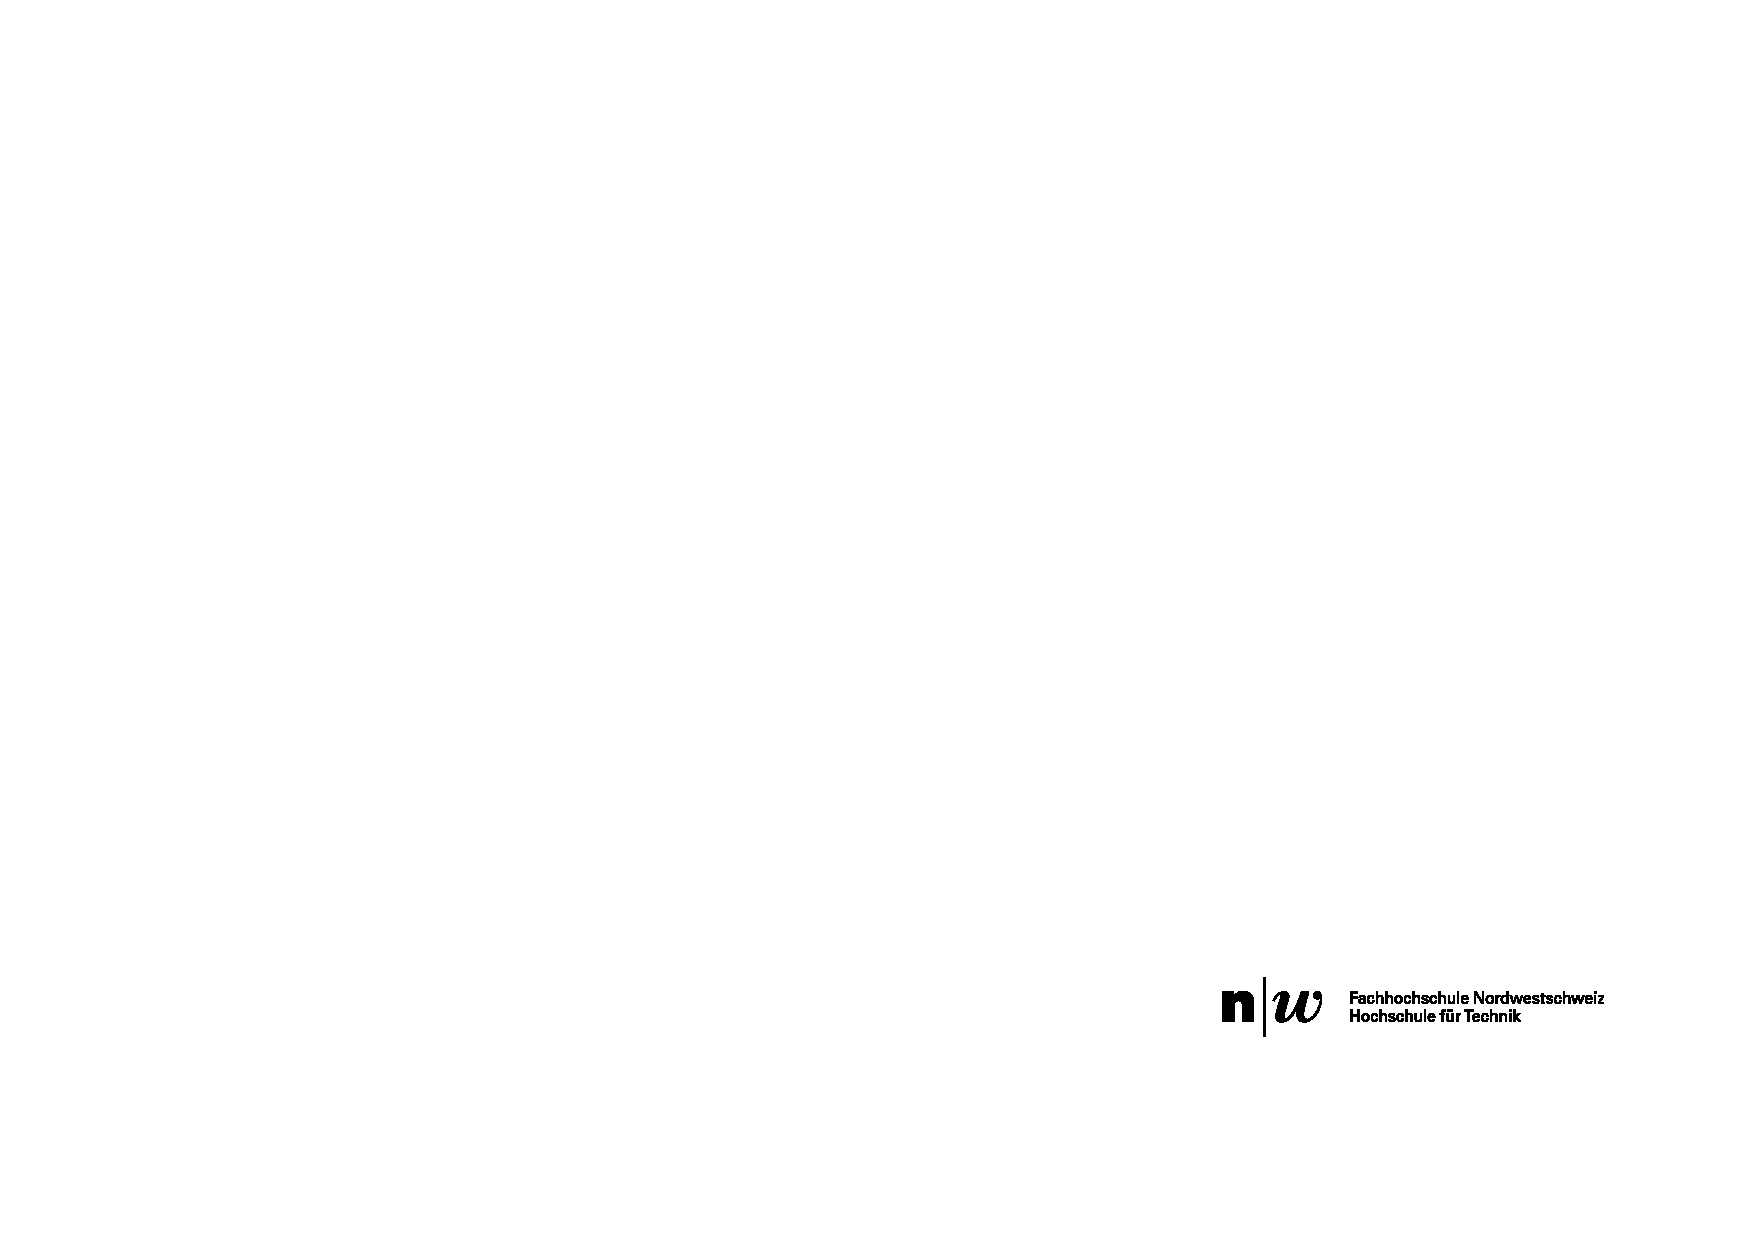
\includegraphics[scale=1]{graphics/fhnw_ht_logo_de.pdf}
	\end{figure}
	\begin{center}
		\vspace*{2cm}
		{\huge{\textbf{\thetitle}}}\\
		\vspace*{1cm}
		
		{\huge{Bachelor Thesis}}\\
		\vspace*{0.5cm}
		
		{\scshape\Large Paper - \theauthor \\} \Large{\today}
		\vspace*{3cm}
		\selectlanguage{english}				%ngerman or english
		\thispagestyle{empty}
		\begin{abstract}
			Among the most popular low power mesh network protocols in free GHz ISM band the three mesh stacks Bluetooth Mesh, ZigBee and Thread are currently competing against each other. The assignment of this bachelor thesis was to build a consistent test framework for all three mesh-networks to benchmark them under realistic conditions. Due to better combability, the nRF52840 SoC from Nordic Semiconductors was the chosen microcontroller for all three network stacks. The benchmark is structured in two parts, a battery powered slave node and a master which is directly connected to a computer. The master node is responsible for controlling the measurement, whereas the slave nodes send benchmark messages to each other. These benchmark messages collect the necessary information to determine latency, RSSI, throughput and active radio time. For a better comparability an apartment house, an apartment and a labor environment were selected as different test benches. The Thread stack results the best in the different test benches. Because of its automatic routing it is able to adapt himself to the environment, as a result the latency of this stack is in every three benches similarly low. Bluetooth Mesh was able to reach the lowest latency with small payload. The ZigBee network stands out with its constant and low latency within one test bench. As a conclusion all of the three networks perform well in case of a home automation. Due to of their own assets and drawbacks it cannot be said this is the best mesh-stack. It depends on the application which mesh network performs the best.
		\end{abstract}

	\end{center}
\clearpage

%%---TABLE OF CONTENTS-------------------------------------------------------------------
%\pagenumbering{Roman}		
%\selectlanguage{ngerman}				%ngerman or english
%\tableofcontents
%\clearpage

%%---TEXT--------------------------------------------------------------------------------
\pagenumbering{arabic}

\clearpage

\section{Einleitung}\label{sec:Einleitung}
Im 2.4GHz ISM-Band konkurrieren sich derzeit die drei weit verbreiteten Low Power Mesh Netzwerk Protokolle Bluetooth Mesh, Thread und Zigbee. Alle drei wurden konzipiert für die kabellose Übertragung in sogenannten WSN (Wireless Sensor Networks) oder in Netzen für die Heim Automatisierung. Während Thread und Zigbee den IEEE 802.15.4 Standard als Physical Layer benutzen basiert der BT Mesh Stack auf dem BLE (Bluetooth Low Energy) Standard. Aufgrund der hohen Dichte an Netzwerkprotokollen die das 2.4GHz ISM-Band ebenso nutzen (z.B. Wifi) sind die Störeinflüsse auf die Mesh Protokolle eines der grössten Probleme. Die Protokollstacks begegnen diesem und weiteren Problemen auf unterschiedliche Weise. Diese Unterschiede und schliesslich die Performance der Mesh Netzwerke sollen unter unterschiedlichen Testbedingungen aufgezeigt werden wodurch ein objektiver Vergleich der drei Mesh Protokolle möglich wird. In der nachfolgenden Tabelle ist sind die Hauptmerkmale der drei verschiedenen Mesh-Netzwerke aufgelistet:

\begin{table}[h]
	\centering
	\begin{adjustbox}{width=1\textwidth}
		\begin{tabular}{@{}|l|l|l|l|@{}}
			\toprule
			\multicolumn{4}{|c|}{\textbf{Mesh Netzwerke im Vergleich}}                                                                                                            \\ \midrule
			& \textbf{Bluetooth Mesh}              & \textbf{Thread}                                  & \textbf{ZigBee}                              \\ \midrule
			\textbf{Markt}               & Beleuchtung und Smart Home           & Industrie und Smart Home                         & Beleuchtung, Haus Automation und Messtechnik \\ \midrule
			\textbf{Veröffentlicht}      & 2017                                 & 2015                                             & 2003                                         \\ \midrule
			\textbf{Appllikations Layer} & Mesh Model System                    & Verknüfpbar mit allen IPv6 basierten Protokollen & Cluster Bibliothek                           \\ \midrule
			\textbf{IPv6}                & Nein                                 & Ja                                               & Nein                                         \\ \midrule
			\textbf{Netzwerk Zugriff}    & Smartphone oder Gateway              & Border Router                                    & Gateway                                      \\ \midrule
			\textbf{Ökosysteme}          & Ledvance                             & Google Nest                                      & Ikea, Phillips Hue, Amazon und weitere       \\ \midrule
			\textbf{Routing}             & Managed Flooding                     & Geroutet                                         & Geroutet                                     \\ \midrule
			\textbf{Weiteres}            & Ist direkt mit Smartphone erreichbar & Automatisiertes Verwalten des Netzwerks          & Am meisten verbreitet                        \\ \bottomrule
		\end{tabular}
	\end{adjustbox}
	\caption{Vergleich Mesh Netzwerke}\label{table:VergleichMeshNetzwerk}
\end{table}

Hauptziel ist ein objektiver Vergleich der drei gängigsten Low Power Mesh Netzwerke Bluetooth Mesh, Thread und Zigbee bezüglich deren Leistungsfähigkeit unter wechselnden Bedingungen. Es soll erkennbar werden, welches Protokoll in welchen Bereichen seine Stärken hat und wie es am besten eingesetzt werden kann. Die detaillierte Behandlung des ganzen Projektes ist im Fachbericht verfügbar.


\pagebreak

\clearpage
\section{Methode}\label{sec:Methode}
Um die Performance der drei Mesh Stacks zu vergleichen wurde ein einheitliches Benchmark Konzept erarbeitet. Dieses definiert die Mesh Parameter, Testumgebungen, den Ablauf sowie sämtliche Messgrössen und Messreihen.

\subsection{Messablauf}
Für den Vergleich der 3 Mesh Netzwerkstacks Bluetooth Mesh (BT Mesh), Thread und Zigbee wird ein vom Mesh Protokoll unabhängiges Testkonzept umgesetzt welches in der Abbildung \ref{fig:KonzeptschemaTestablauf} als Konzeptschema dargestellt ist. Die Benchmark Slave Nodes (BSN) in der Abbildung als Sensoren und Aktoren mit unterschiedlichen Funktionalitäten dargestellt, bilden zusammen mit dem Benchmark Master Node (BMN) das zu testende Mesh Netzwerk. Innerhalb des Netzwerks wird dessen Organisation vom jeweiligen Protokoll sichergestellt. Das Testnetzwerk soll ein realitätsnahes Netzwerk nachbilden. Beispielsweise wird eine Hausautomation in einem Einfamilienhaus als Referenz angenommen in welchem jeweils nur gewisse Nodes untereinander Applikationsdaten austauschen. Ein Lichtschalter kommuniziert nur mit einer Lichtquelle und umgekehrt. Der selbe Lichtschalter tauscht jedoch keine Applikationsdaten mit dem Temperatursensor aus. Trotzdem bilden die Nodes zusammen ein Mesh Netzwerk.\\

Die Benchmark Management Station (BMS) welche mit dem BMN via USB/UART kommuniziert, ist zuständig für die Verwaltung und Verarbeitung der Benchmarks. Während eines Benchmark Prozesses sollen sämtliche Messungen jedoch unabhängig von der BMS durchgeführt werden damit allfällige Latenzzeiten der USB/UART Verbindung die Resultate nicht verfälschen.

\begin{figure}[h]
	\centering
	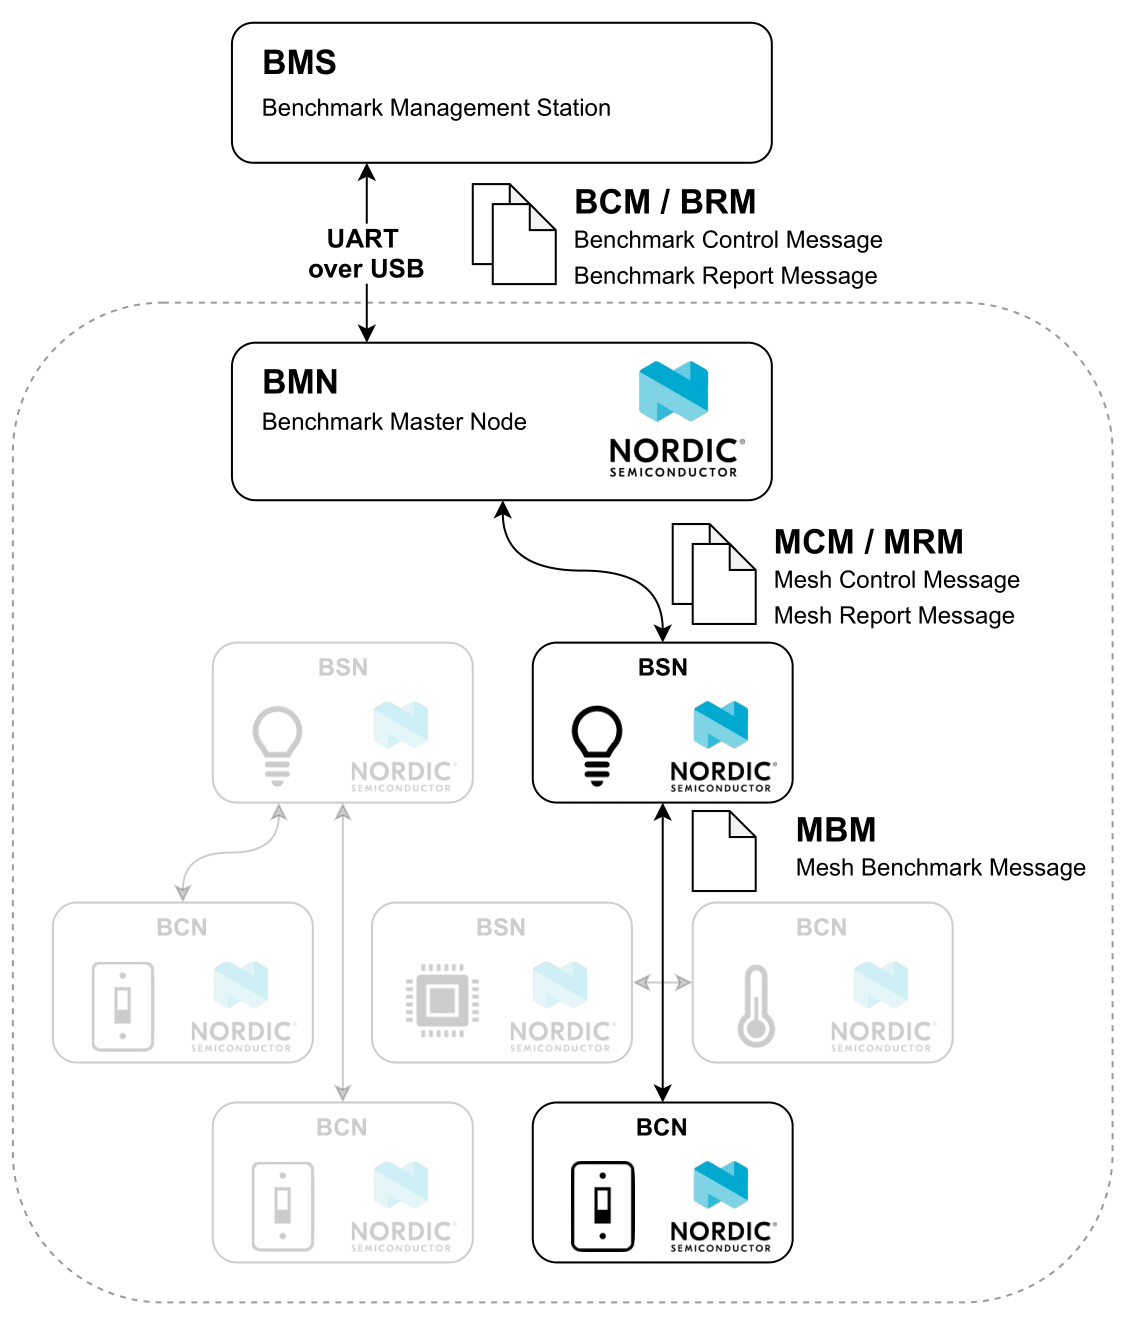
\includegraphics[width=0.55\textwidth]{graphics/Mesh_Testkonzeptschema.png}
	\caption{Konzeptschema Testablauf}
	\label{fig:KonzeptschemaTestablauf}
\end{figure}

\newpage
\subsection{Messaufbau}
Unterschiedliche Testumgebungen sollen die Benchmarks und schlussendlich den Vergleich der 3 Mesh Protokolle aussagekräftiger machen. Nachfolgende Umgebungen mit den entsprechenden Eigenschaften sollen getestet werden. Die Abbildungen zu den Testumgebungen zeigen jeweils die Platzierung der Nodes sowie deren Funktion und Gruppen Zugehörigkeit. Die Farbe Grün identifiziert den Node als Client Node während Blau für einen Server Nodes steht. Die Nummerierung zeigt welcher Node zu welcher Adressgruppe gehört. Ein Client Node in Gruppe 1 sendet jeweils Nachrichten zu allen Server Nodes in der selben Gruppe. 
\newline

\paragraph{Labor}
\begin{wrapfigure}{r}{0.6\textwidth}
	\centering
	\vspace{-20pt}
	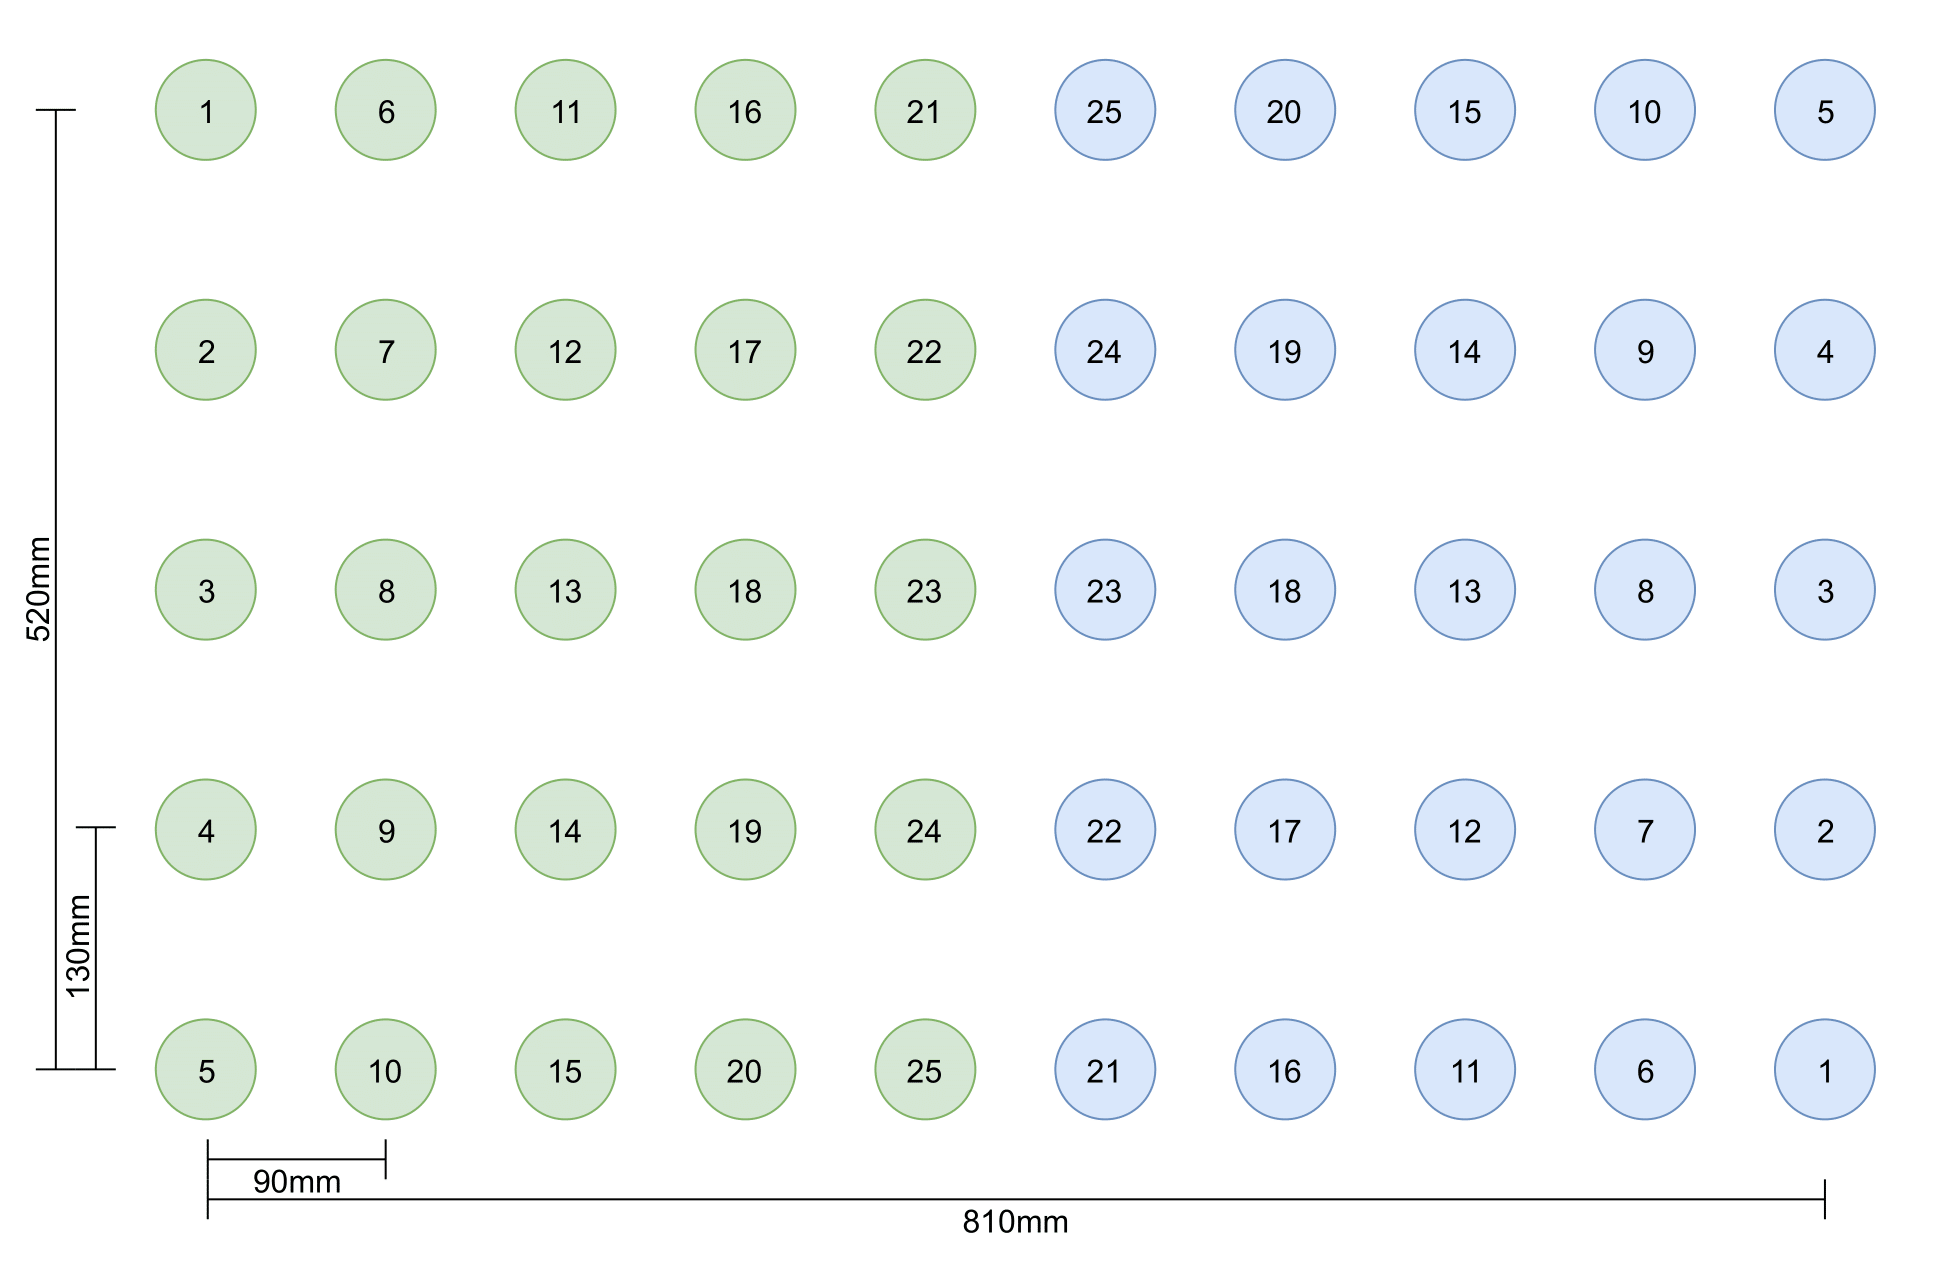
\includegraphics[width=0.6\textwidth]{graphics/Testaufbau_Labor.png}
	\caption{Testaufbau Labor}
	\label{fig:TestaufbauLabor}
	\vspace{-10pt}
\end{wrapfigure}
Der Laboraufbau ist ein Extremtest welcher die Leistungsgrenzen der Protokollstacks ausloten soll. Dabei werden die Nodes auf einem Raster gemäss Abbildung \ref{fig:TestaufbauLabor} angeordnet. Die genauen Abmessungen sind der Abbildung zu entnehmen.
\vspace{40mm}

\paragraph{Einfamilienhaus}
\begin{wrapfigure}{r}{0.6\textwidth}
	\centering
	\vspace{-105pt}
	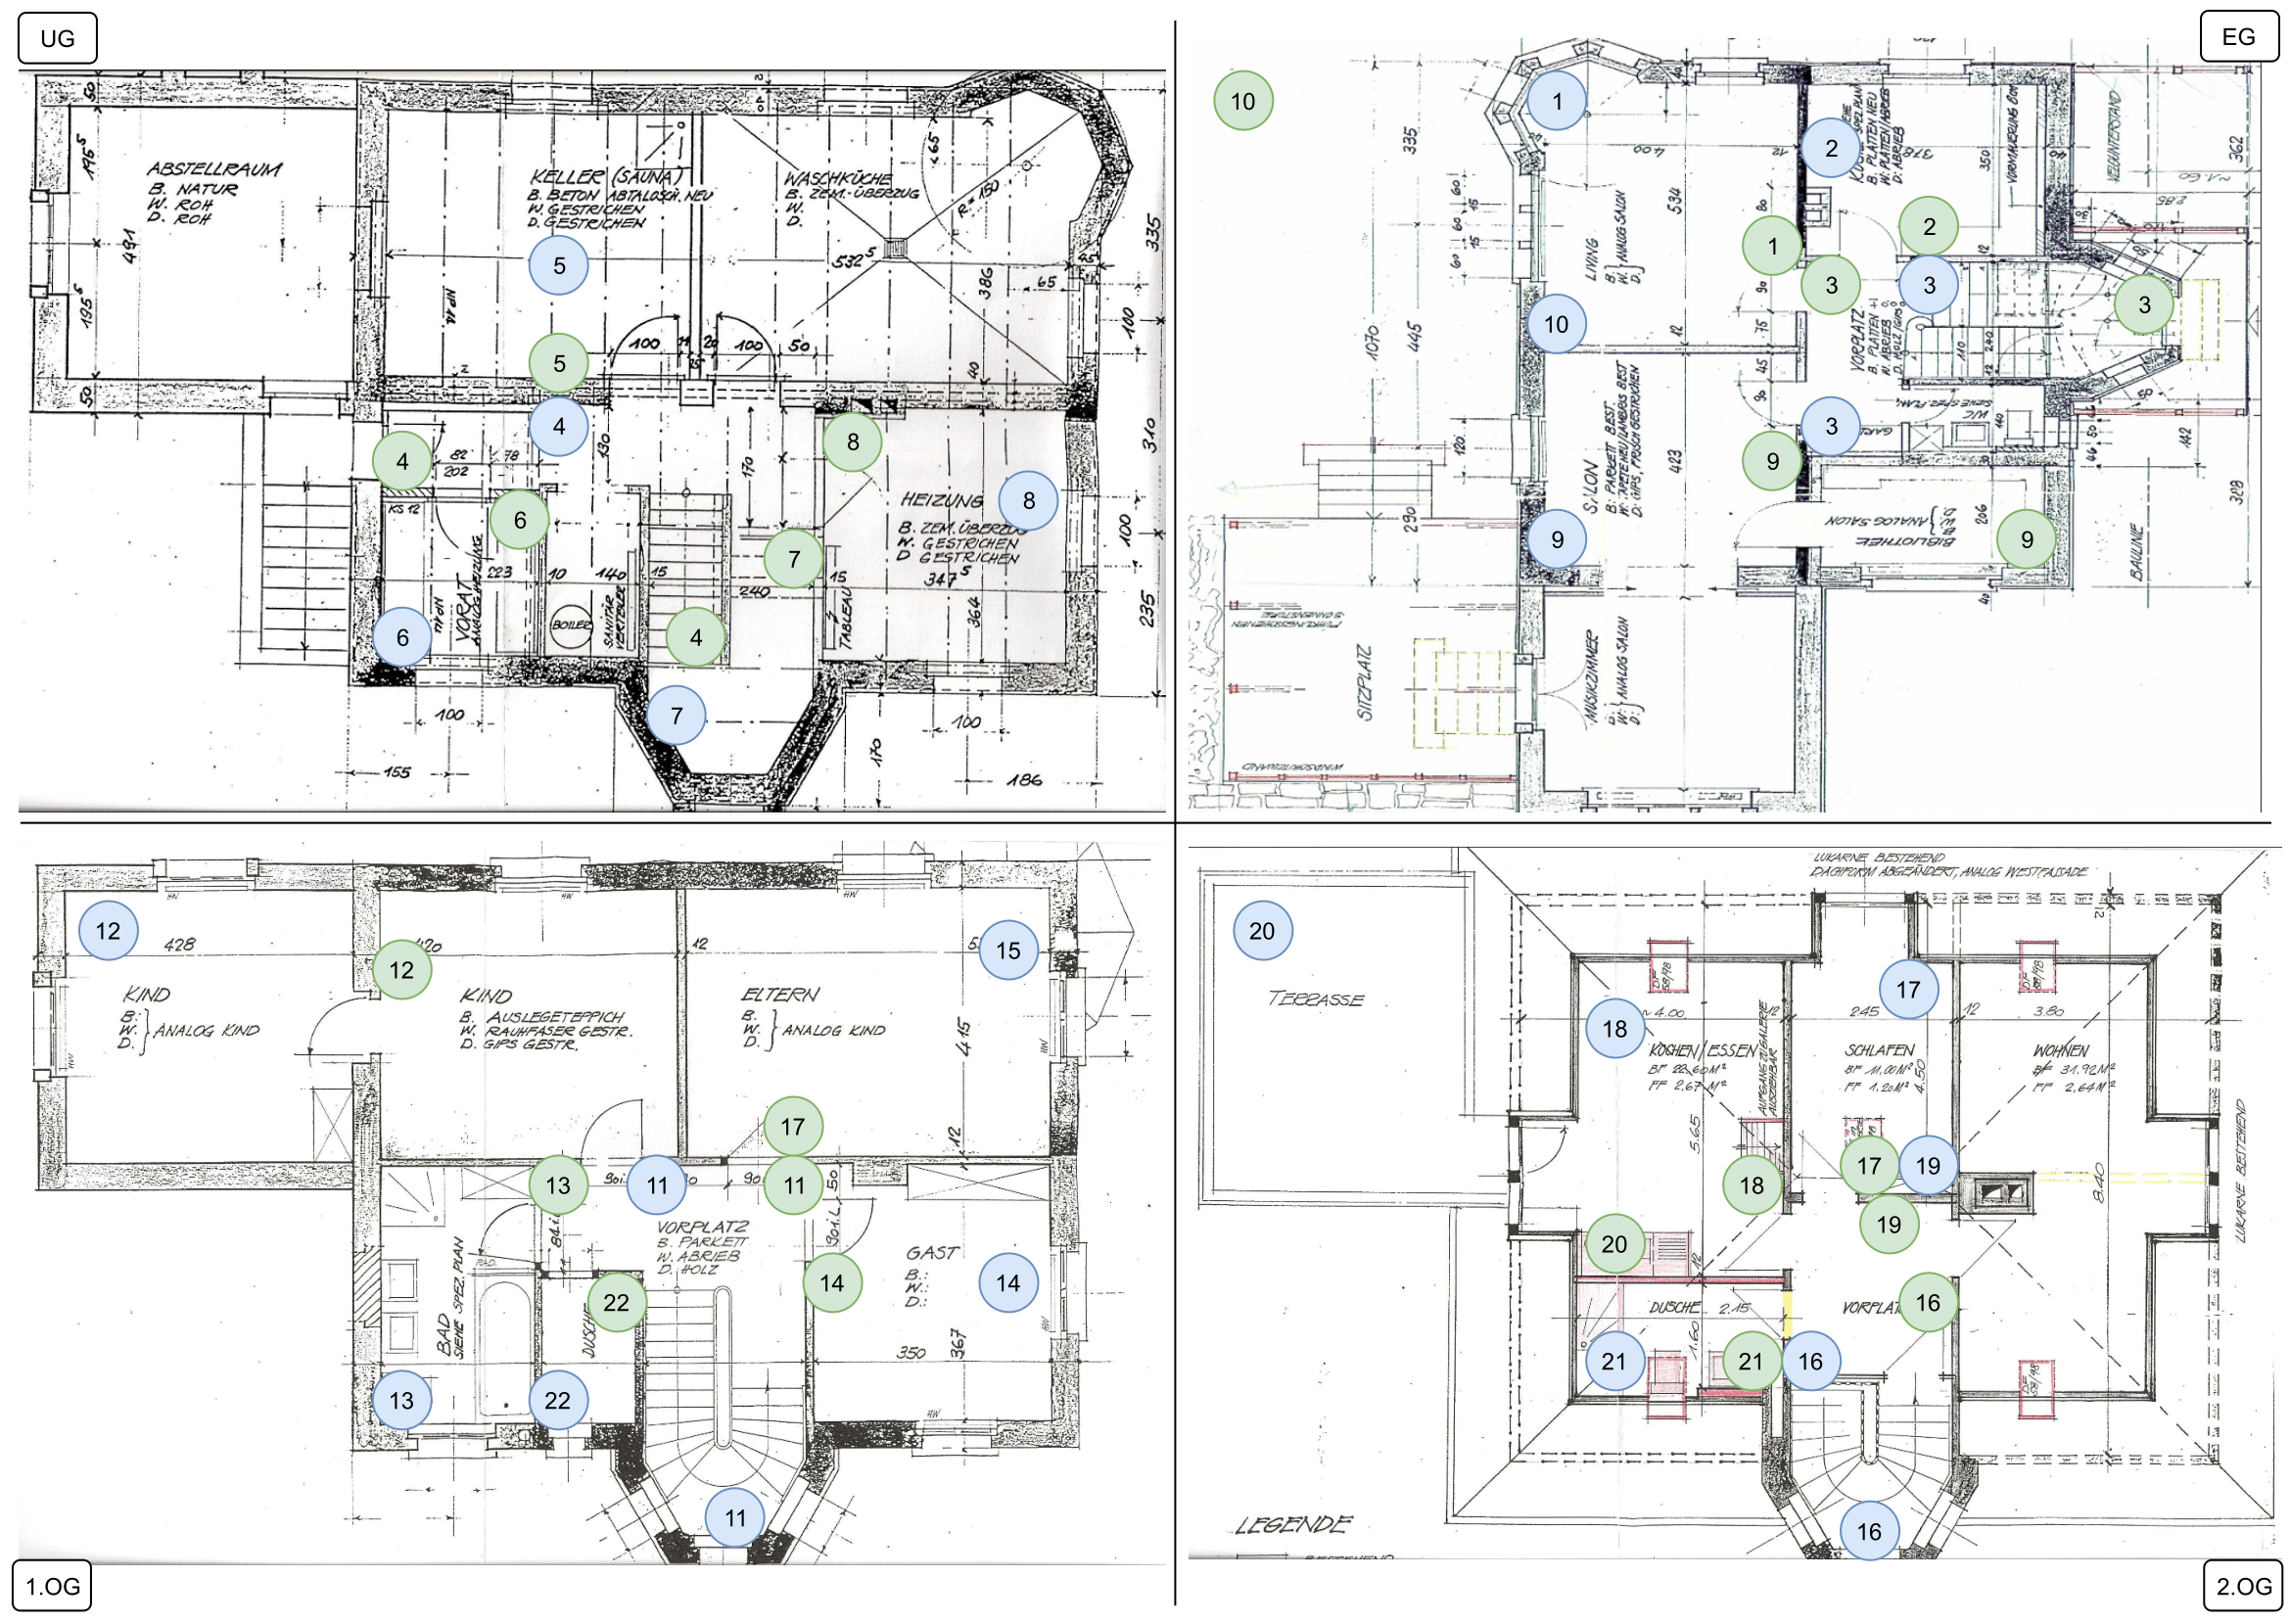
\includegraphics[width=0.6\textwidth]{graphics/Plan_Haus_Raffi.png}
	\caption{Platzierung der Nodes im Einfamilienhaus}\label{fig:Messumgebung2Einfamilienhaus}
	\vspace{-50pt}
\end{wrapfigure}
Die Testgeräte werden in einem Einfamilienhaus installiert und repräsentieren damit eine flächendeckende Heim-Automatisierung. Folgende Eingenschaften soll diese Messung abdecken:

Die Abbildung \ref{fig:Messumgebung2Einfamilienhaus} zeigt den Schnitt des Einfamilienhauses in welchem der Benchmark durchgeführt wurde.

\newpage
\paragraph{Wohnung}
\begin{wrapfigure}{r}{0.6\textwidth}
	\centering
	\vspace{-80pt}
	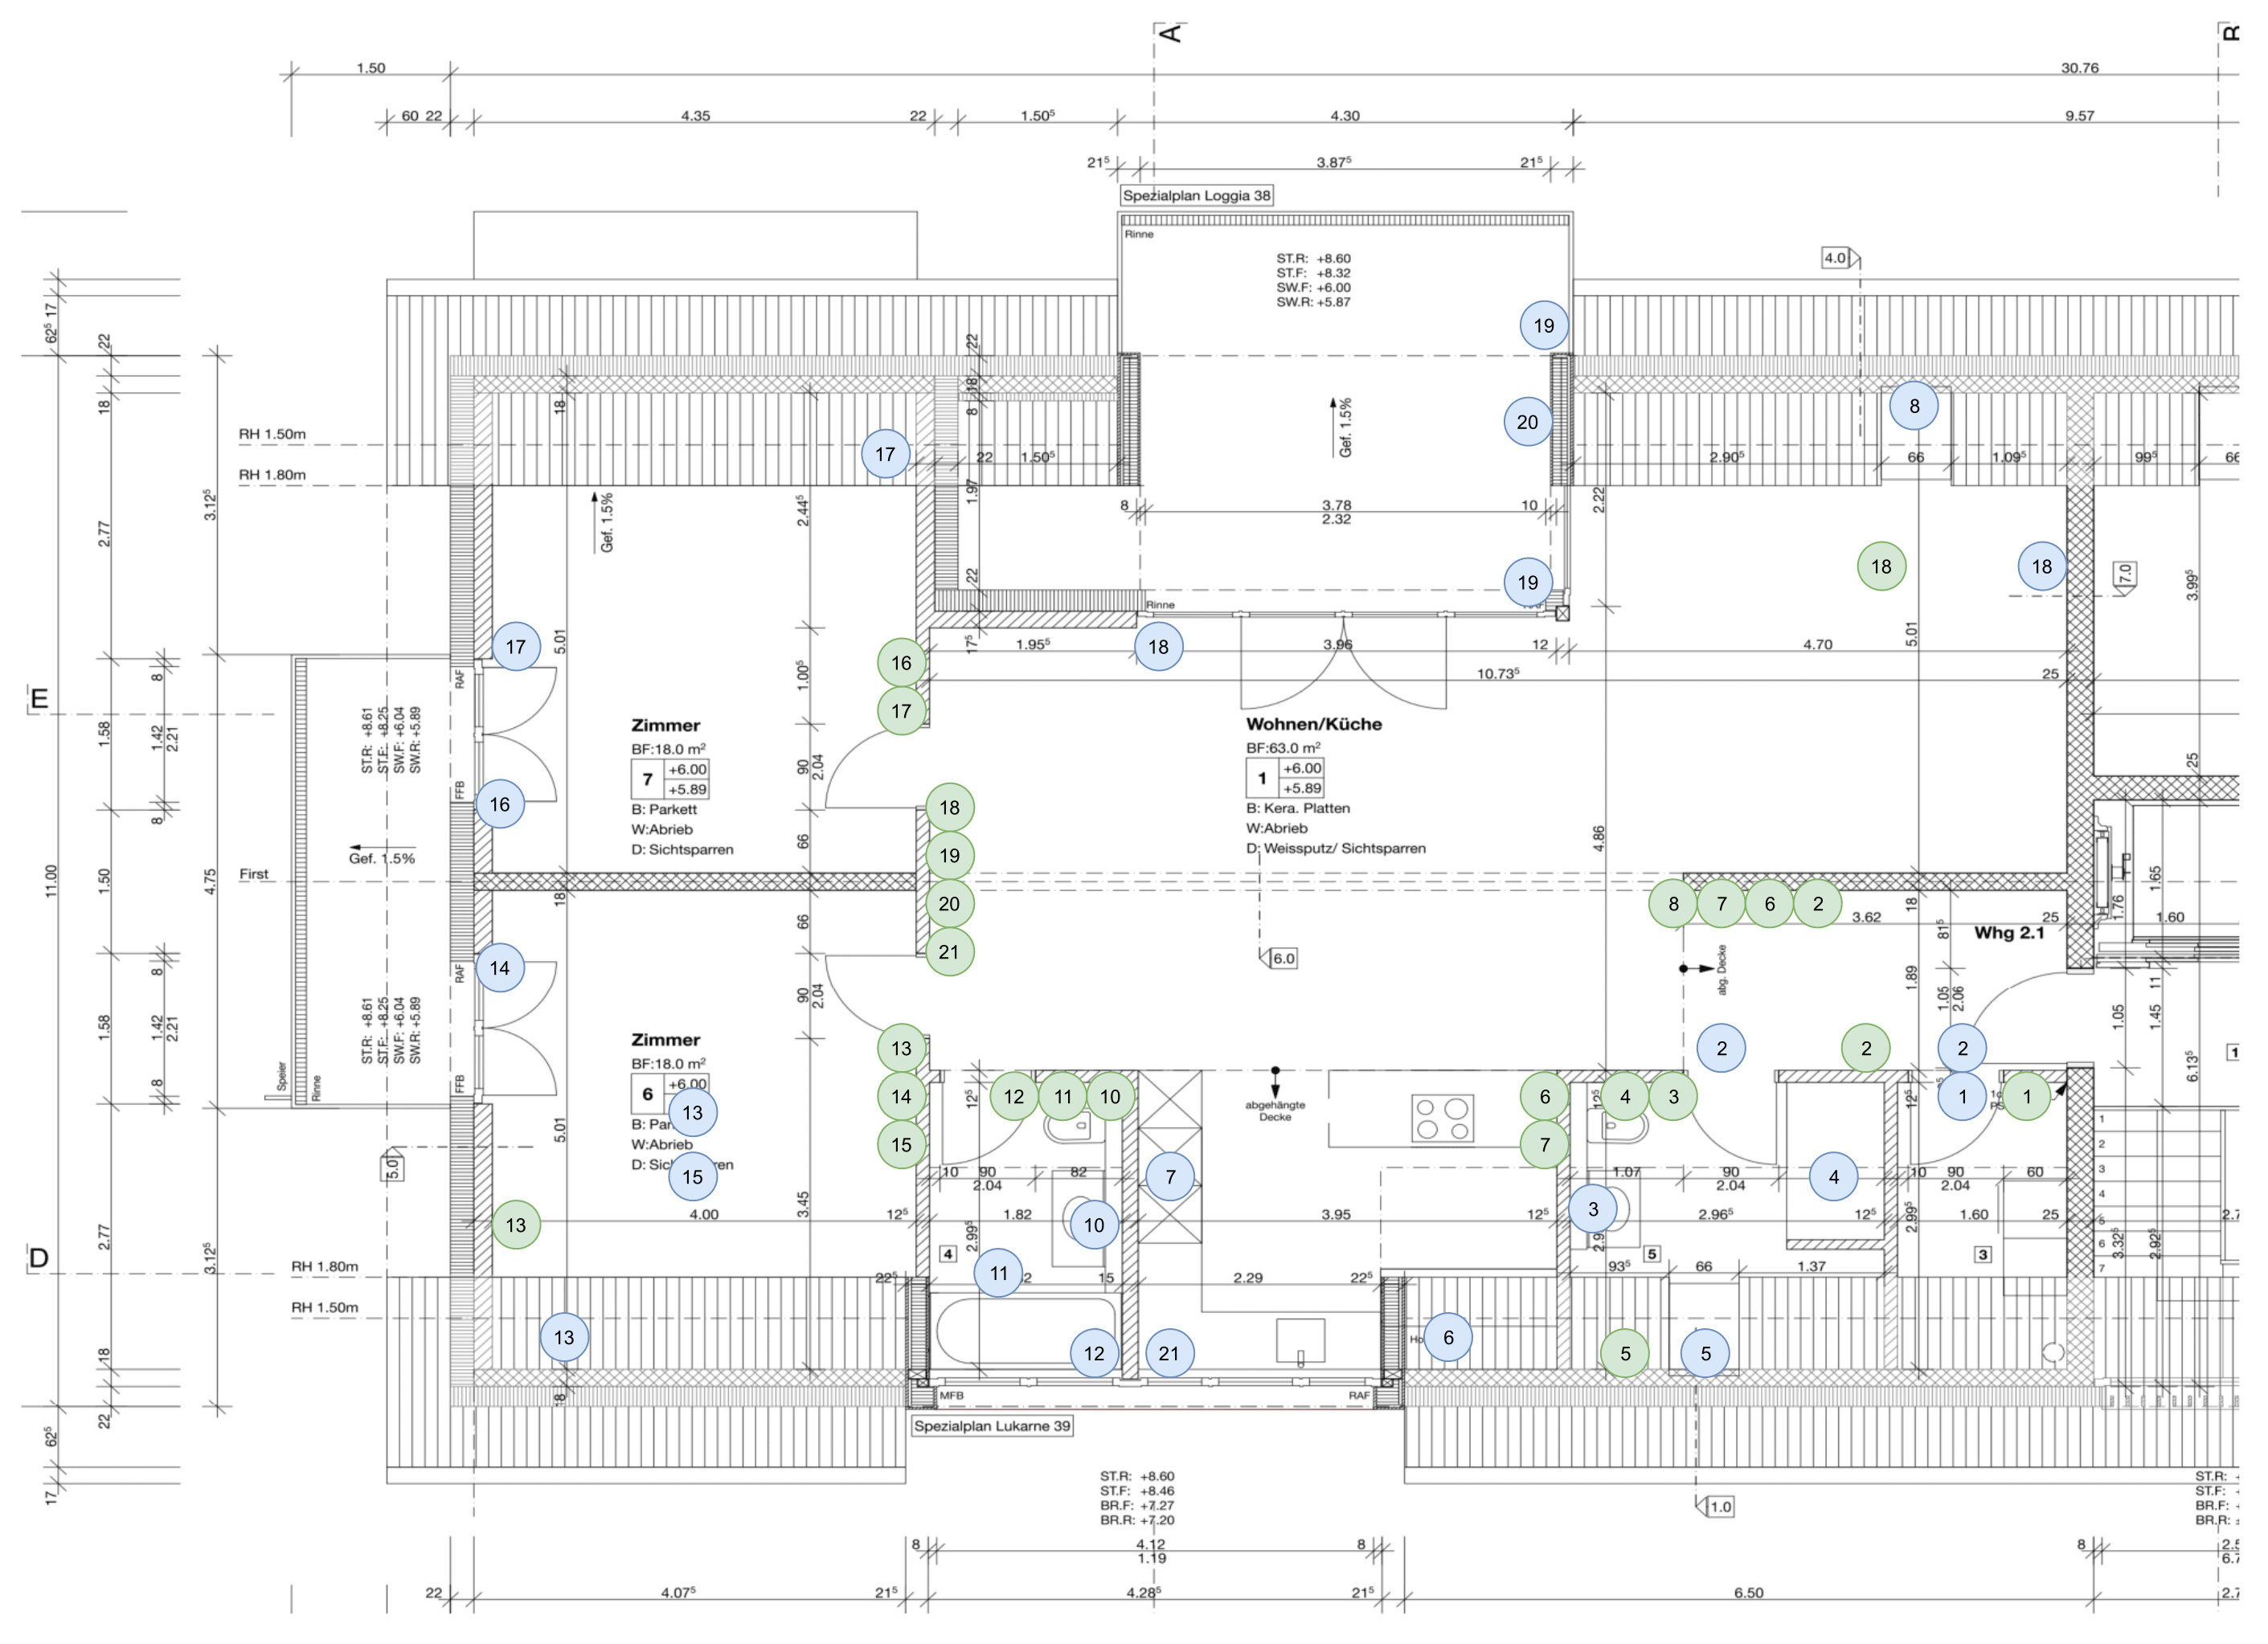
\includegraphics[width=0.6\textwidth]{graphics/Plan_Wohnung_Cyrill_Nodes_Placement.png}
	\caption{Testaufbau Wohnung}
	\label{fig:TestaufbauWohnung}
	\vspace{-100pt}
\end{wrapfigure}
Ebenfalls als Heim-Automatisierung gedacht werden die Messungen in einer Wohnung durchgeführt.

Bei der Wohnung handelt es sich um eine 3.5 Zimmer Wohnung mit einer Wohnfläche von 122 Quadratmetern. Die genauen Abmessungen sowie die Platzierung der Nodes ist in Abbildung \ref{fig:TestaufbauWohnung} zu sehen.

\vspace{30mm}
\subsection{Vergleichswerte und Messgrössen}\label{subsec:VergleichswerteundMessgrössenMesh}

\subsection{Messerwartung}
Da die Nachrichtenzustellung durch das Routing effizienter realisiert werden kann wird erwartet, dass die beiden auf dem IEEE 802.15.4 Standard aufbauenden Protokolle klare Vorteile haben werden. Hingegen könnte BT Mesh Vorteile haben bei kleiner Belastung des Netzes.

Das menschliche Auge ist in der Lage eine Verzögerung festzustellen, wenn die Latenz vom Knopfdruck bis das Licht angeht mehr als 200ms beträgt. In einer modernen Hausautomation darf natürlich keine Verzögerung wahrgenommen werden. Somit wird erwartet, dass die Latenzzeit im Schnitt unter 200ms bleiben soll. \cite{silicon_laboratories_inc_an1142_2020}
\pagebreak

\clearpage
\section{Ergebnisse}\label{sec:Ergebnisse}
Die Abbildungen \ref{fig:VerteilungderLatenzzeiten} bis \ref{fig:OngoingTransactions} zeigen die Messresultate der Messung 2 in der Messumgebung \textit{Wohnung}. Sie stehen exemplarisch für die Messergebnisse aller Messreihen.
In Abbildung \ref{fig:VerteilungderLatenzzeiten} ist die prozentuale Verteilung der Latenzzeiten pro Hop dargestellt.
In sämtlichen Grafiken werden die Ergebnisse von BT Mesh in blau, jene von Thread in grün und jene von Zigbee in rot dargestellt.
So ist ein direkter Vergleich der Protokolle möglich.
Abbildung \ref{fig:VerteilungderLatenzzeiten} sagt also aus wie viele Nachrichten das Ziel mit einer bestimmten Latenzzeit erreicht haben.
Nachrichten die das Ziel nicht erreicht haben, also Pakete die verloren gegangen sind, werden dabei nicht berücksichtigt.
Im gezeigten Beispiel haben rund 76 Prozent der Nachrichten die im BT Mesh Test versendet wurden das Ziel mit einer maximalen Latenzzeit von 10 Millisekunden erreicht.
Die weitere Verteilung geht bis auf Latenzzeiten von über 300 Millisekunden wobei die Prozentzahl der Nachrichten in diesem Bereich sehr tief ist.
Die Werte für Thread und Zigbee zeigen hingegen eine deutlich schmalere Verteilung der Latenzzeiten.
Aus den in Abbildung \ref{fig:VerteilungderLatenzzeiten} aufgezeigten Latenzzeiten wurde der Durchschnitt gebildet und in Abbildung \ref{fig:DurchschnittlicheLatenzzeit} dargestellt.
Es handelt sich dabei wiederum um die Latenzzeit pro Hop. Im Falle von Zigbee ist dies erwähnenswert, da hier die Anzahl Hops nicht ausgelesen werden konnte und die Resultate somit mit Vorsicht interpretiert werden müssen. Mehr dazu in der Validierung im Abschnitt \ref{subsec:Validierung}.

\begin{figure}[h]
	\centering
	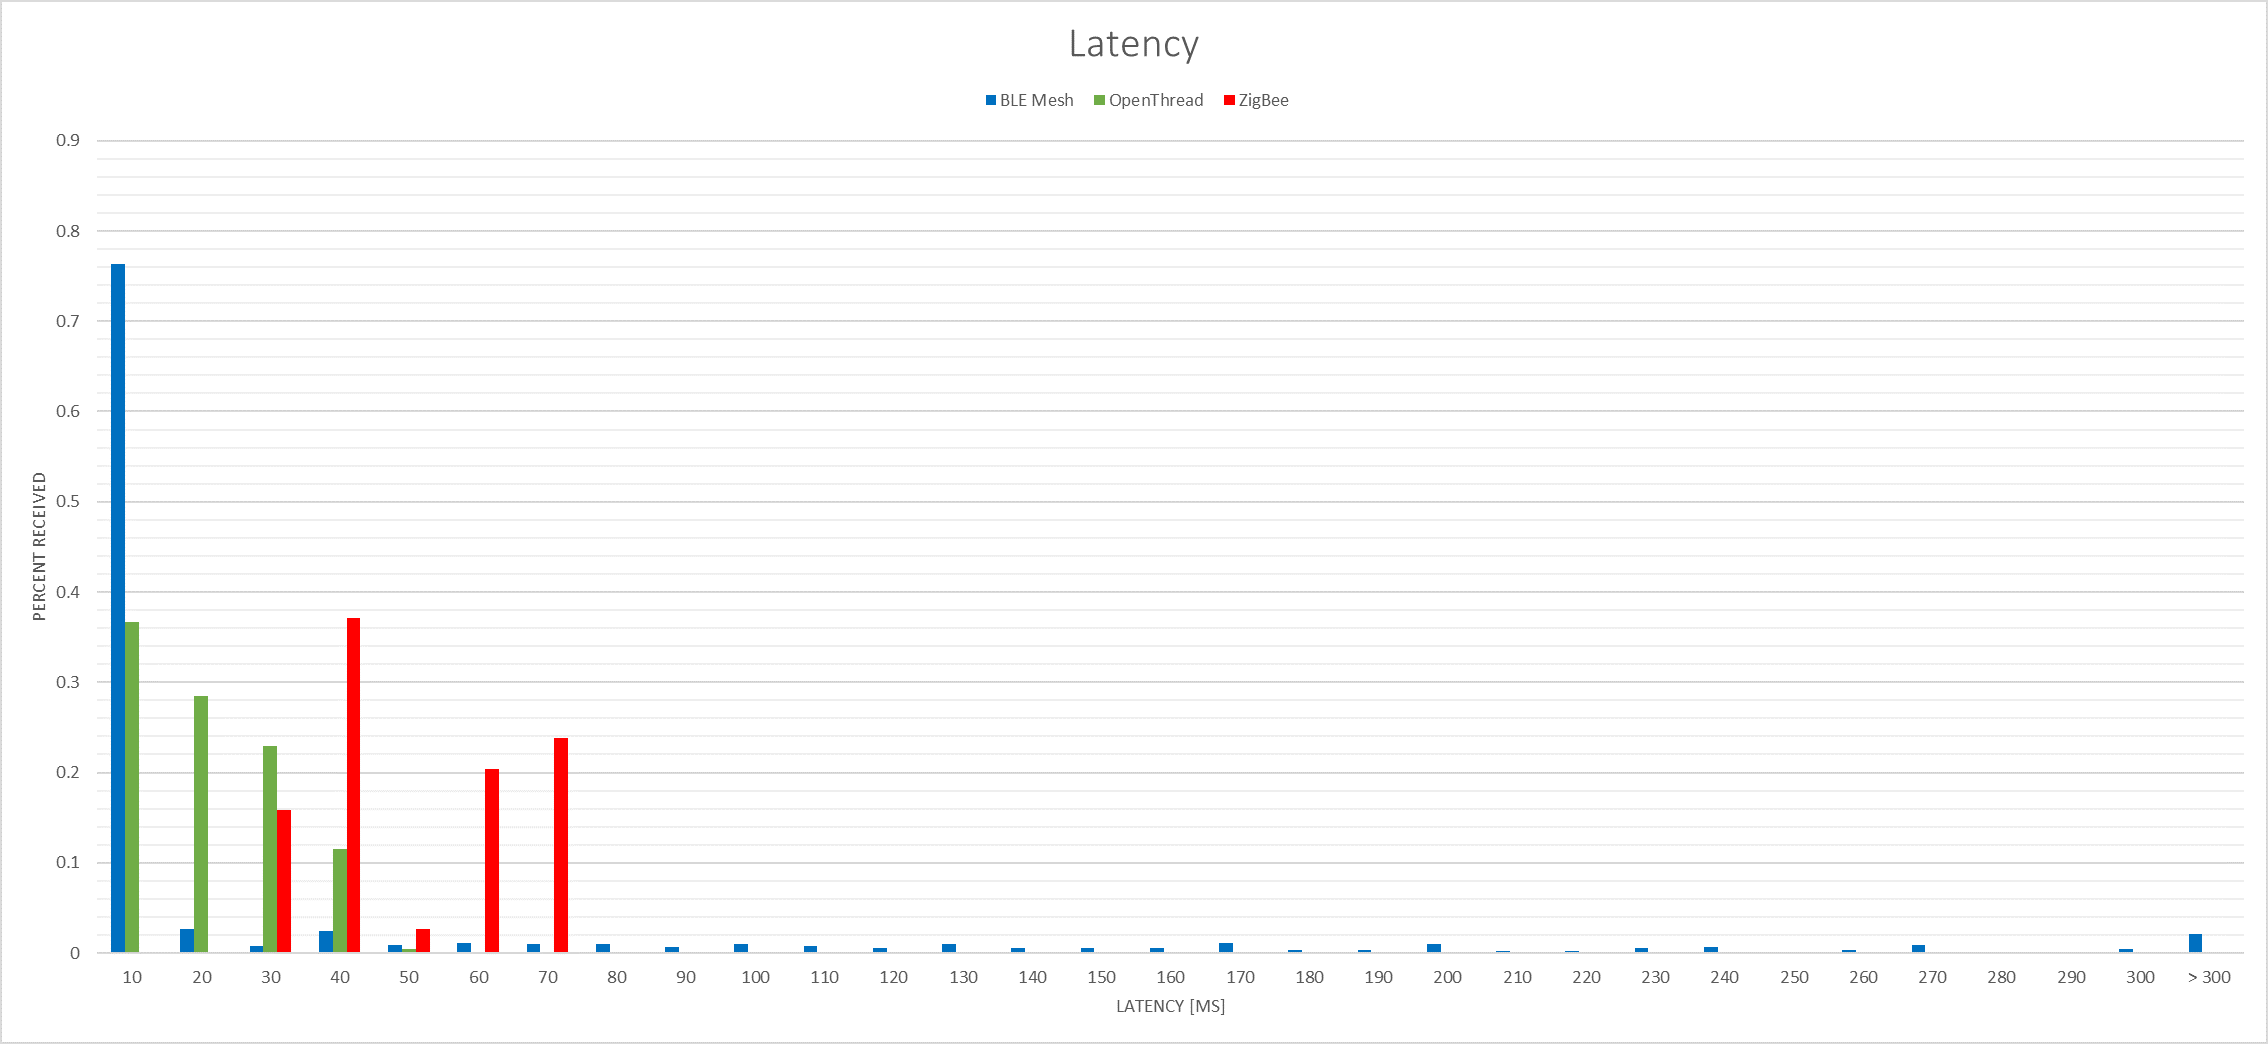
\includegraphics[width=\textwidth]{Latency_2_Wohnung.png}
	\caption{Messung 2 Wohnung: Verteilung der Latenzzeiten pro Hop}
	\label{fig:VerteilungderLatenzzeiten}
\end{figure}

\newpage
Der durchschnittliche Datendurchsatz der mit der Abbildung \ref{fig:DurchschnittlicherDurchsatz} aufgezeigt wird, muss mit der selben Vorsicht betrachtet werden. Denn auch hier werden die Werte pro Hop für die Berechnung verwendet.
Die präsentierten Werte werden errechnet aus der Paketgrösse und der Latenzzeit des übertragenen Pakets.
Dabei werden die Werte für den Durchsatz für jedes empfangene Paket berechnet und davon schliesslich der Mittelwert gebildet und in Abbildung \ref{fig:DurchschnittlicherDurchsatz} dargestellt.
Die oben erwähnten Ausreisser bei BT Mesh bewirken nun einen unerwartet hohen Durchsatz bei BT Mesh im Vergleich zu jenem bei Thread welches konstant tiefe Latenzzeiten hat.

\begin{figure}[!htbp]
	\centering
	\begin{minipage}[b]{0.49\textwidth}
		\centering
		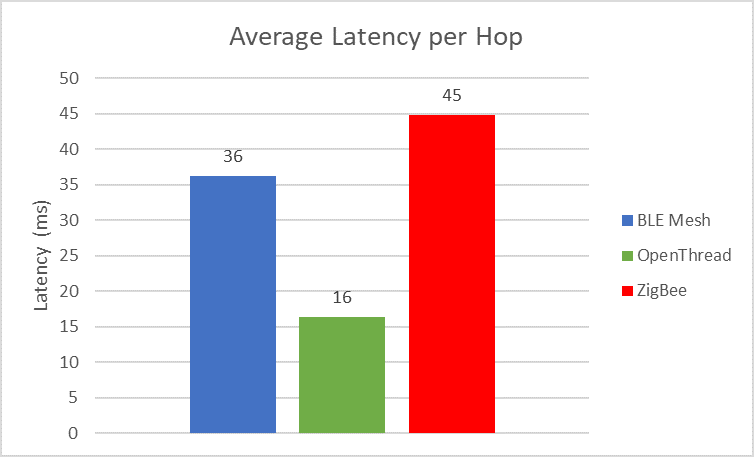
\includegraphics[width=\textwidth]{Average_Latency_per_Hop.png}
		\caption{Messung 2 Wohnung: Durchschnittliche Latenzzeit pro Hop}
		\label{fig:DurchschnittlicheLatenzzeit}
	\end{minipage}
	\begin{minipage}[b]{0.49\textwidth}
		\centering
		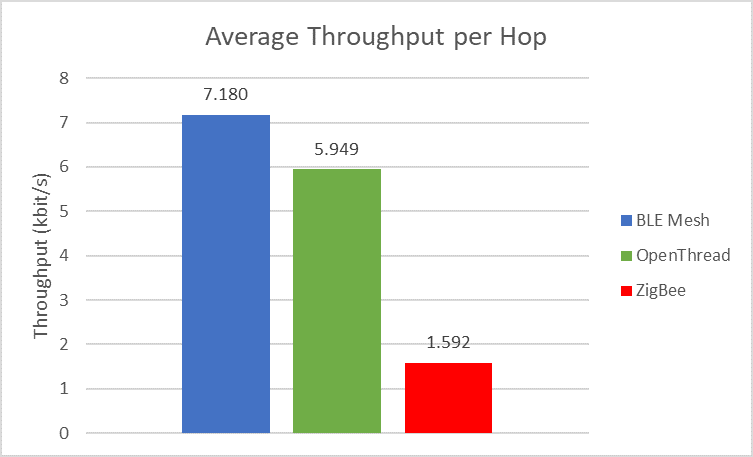
\includegraphics[width=\textwidth]{Average_Throughput_per_Hop.png}
		\caption{Messung 2 Wohnung: Durchschnittlicher Durchsatz pro Hop}
		\label{fig:DurchschnittlicherDurchsatz}
	\end{minipage}
\end{figure}

In der Abbildung \ref{fig:DurchschnittlicherPaketverlust} wird der prozentuale Paketverlust gezeigt über die gesamte Anzahl Nachrichten die während dem Benchmark versendet wurden.
Die Paketverluste von einzelnen Client-Server Beziehungen werden nicht separat ausgewertet.
Wiederum im Beispiel von BT Mesh sind in dieser Messung 2.07 \% der Pakete nicht am Ziel angekommen.

\begin{figure}[!htbp]
	\centering
	\begin{minipage}[b]{0.49\textwidth}
		\centering
		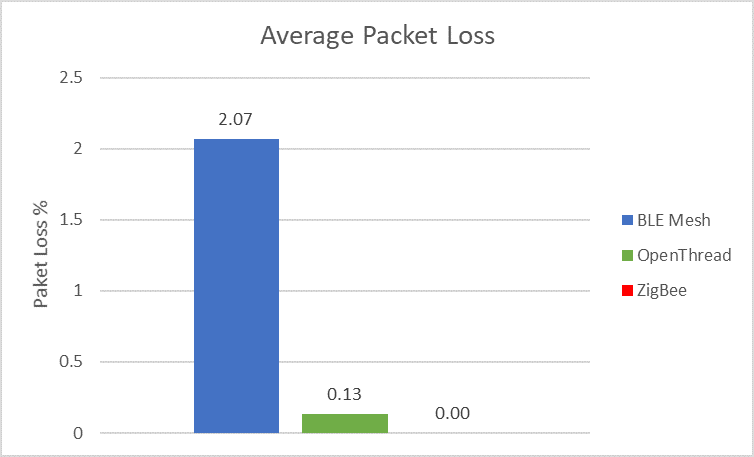
\includegraphics[width=\textwidth]{Average_Packet_Loss.png}
		\caption{Messung 2 Wohnung: Durchschnittlicher Paketverlust}
		\label{fig:DurchschnittlicherPaketverlust}
	\end{minipage}
	\begin{minipage}[b]{0.49\textwidth}
		\centering
		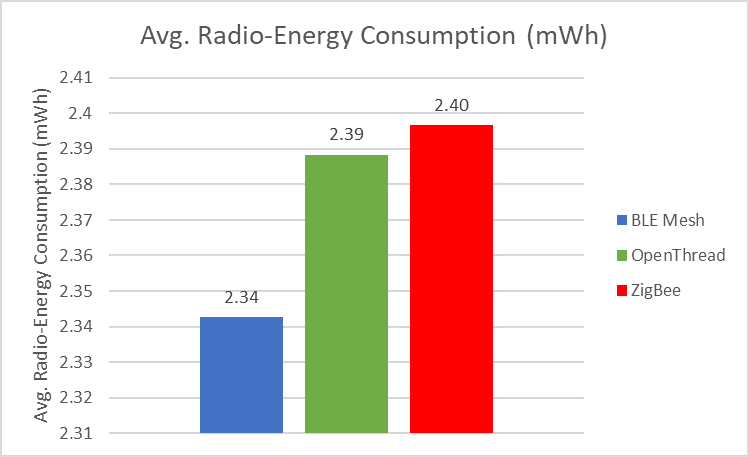
\includegraphics[width=\textwidth]{Average_Radio_Energy_Consumption.png}
		\caption{Messung 2 Wohnung: Durchschnittlicher Energieverbrauch}
		\label{fig:DurchschnittlicherEnergieverbrauch}
	\end{minipage}
\end{figure}

Mit dem Diagramm in Abbildung \ref{fig:DurchschnittlicherEnergieverbrauch} wird schliesslich noch der durchschnittliche Energieverbrauch der Protokolle dargestellt.
Dieser ist abgeleitet aus der \textit{Active Radio Time} welche direkt auf dem nRF52840 SoC mit der entsprechenden API ausgelesen werden kann.
Die \textit{Active Radio Time} wurde schliesslich mit dem Strombedarf des SoC's bei definierter Speisesannung von 3V verrechnet.
Gemäss den Angaben der Dokumentation von Nordic Semiconductors, beträgt der Strombedarf bei aktivem Funkmodul im Sendemodus 4.8mA.
Eine solche Berechnung erlaubt einen qualitativen Vergleich des Energiebedarf unter den 3 Protokollen da die Umsetzung auf der gleichen Hardware erfolgte.
Die Werte in der Abbildung \ref{fig:DurchschnittlicherEnergieverbrauch} sind jedoch keine quantitativen Verbrauchswerte und können deshalb nur im Kontext des Vergleichs verwendet werden.
Der Strombedarf sämtlicher Peripherie wurde nicht berücksichtigt da dieser prinzipiell bei allen Protokollen identisch ist.

\newpage
Die letzte Grafik gemäss Abbildung \ref{fig:OngoingTransactions} zeigt den Verlauf der \textit{Ongoing Transactions} sowie der Latenzzeiten über die Gesamtdauer einer Messung.
In diesem Fall beträgt die Dauer 600 Sekunden.
Die Grafik soll einen Eindruck darüber vermitteln, wie die Stacks damit umgehen, wenn vielen Nachrichten zur selben Zeit versendet werden.
Die \textit{Ongoing Transactions} welche als durchgezogene Linien dargestellt sind, zeigen zu welchem Zeitpunkt wie viele Nachrichten in der Übermittlung sind.
Da die Nachrichten in diesem Beispiel sequentiellen versendet werden gibt es nur sehr geringe Ausschläge welche im unteren Bildrand zu sehen sind.
Die logarithmische Darstellung der Latenzzeiten als gestrichelte Linie bestätigt die Beobachtungen die in der Abbildung \ref{fig:VerteilungderLatenzzeiten} bereits gemacht wurden.
Zigbee wie auch Thread weisen einen ziemlich regelmässigen Verlauf der Latenzzeiten auf.
BT Mesh hingegen zeigt starke Ausreisser.

\begin{figure}[H]
	\centering
	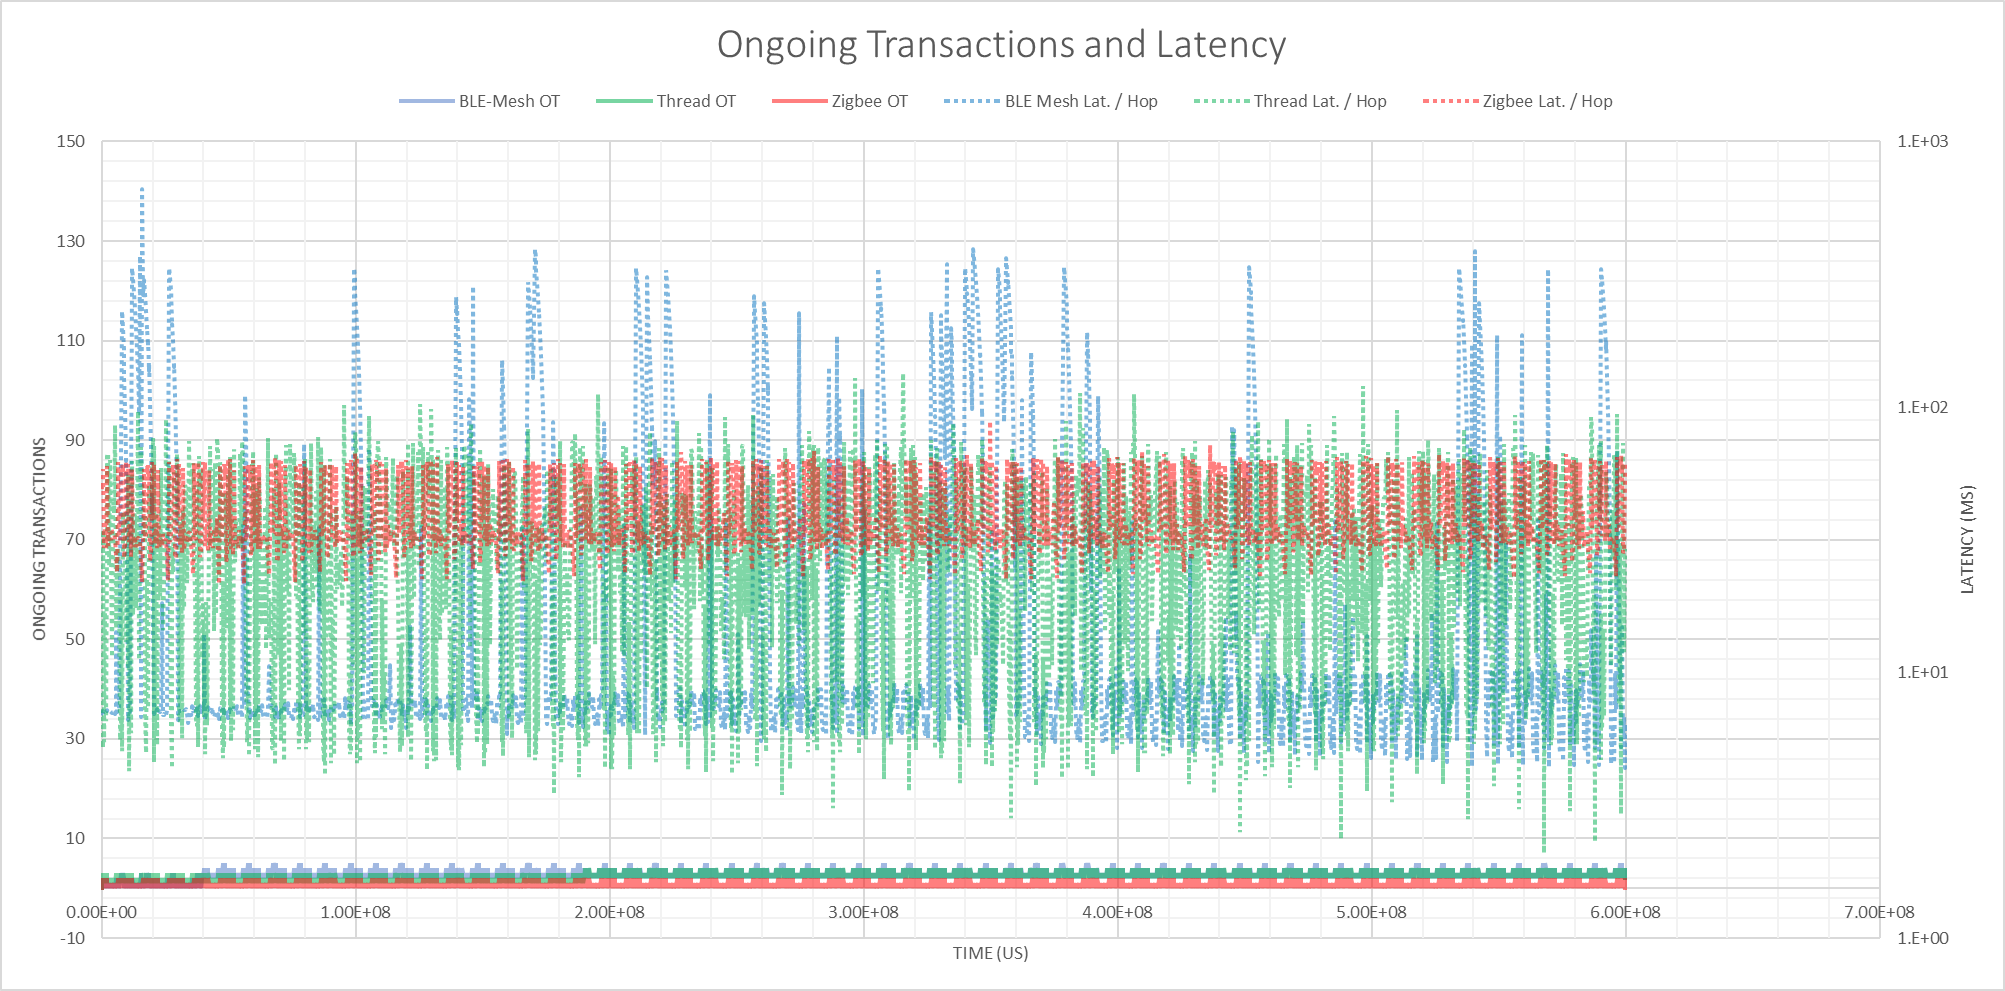
\includegraphics[width=\textwidth]{Ongoing_Transactions_and_Latency.png}
	\caption{Messung 2 Wohnung: Ongoing Transactions und Verlauf der Latenzzeiten über die Messdauer.}
	\label{fig:OngoingTransactions}
\end{figure}
\pagebreak

\clearpage
\section{Interpretation}\label{sec:Interpretation}
Eine Messung unterscheidet sich durch die unterschiedlichen Messparameter, sowie durch den Messaufbau (Wohnung / Labor / Haus). Um einen Vergleich ziehen zu können, wird daher nach diesen beiden Hauptmerkmalen unterschieden.

Dieser Vergleich bezieht sich auf die selbe Testumgebung, jedoch mit unterschiedlichen Messreihen. Im Anschluss soll gezeigt werden wie sich die einzelnen Mesh-Netzwerke bei veränderten Messreihen verändern. Durch die in Abbildung \ref{fig:Latenzzeiten_per_Hop_Messreihen} dargestellten Latenzzeiten wird ersichtlich das Bluetooth-Mesh am anfälligsten auf die Erhöhung der Payload reagiert. Eine detaillierte Analyse zu diesem Phänomen wird in Abschnitt \ref{subsubsec:FazitBluetoothMesh} durchgeführt. Die Verzögerung bleibt bei Zigbee und Thread trotz Erhöhung der Paketlänge stabil. Ein Änderung des Traffic Generation Mode von Random auf Sequentiell bewirkt bei Bluetooth-Mesh eine drastische Abnahme der Latenz. Bei Zigbee ist zwischen der Messreihe 1 und 2 ebenfalls eine Abnahme zu verzeichnen, welche jedoch nicht zwischen der Reihe 3 und 4 feststellbar ist. Somit muss ein anderer Einfluss für die Abnahme verantwortlich sein (in Abschnitt \ref{subsubsec:FazitZigbee} untersucht). Die Änderung des Traffic Generation Mode wirkt bei Thread ebenfalls zu einer Verbesserung der Latenz. Das Senken der Message Dichte führt bei Bluetooth-Mesh zu einer markanten Abnahme der Latenz. Bei Thread und Zigbee bleibt die Latenz nahezu identisch. Die Einbringung von Störungen hat lediglich bei Bluetooth-Mesh einen negativen Einfluss, wodurch sich die Latenzzeit erhöht. 

\begin{figure}[H]
	\centering
	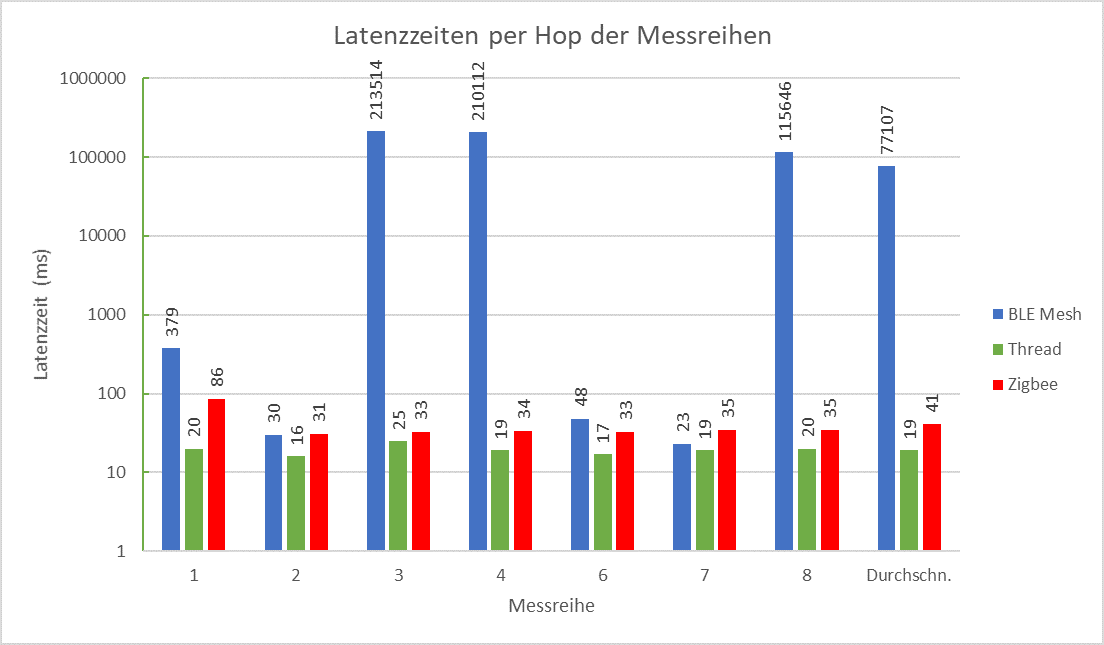
\includegraphics[width=1.0\textwidth]{Latenzzeiten_per_Hop_Messreihen.png}
	\caption{Durchschnittliche Latenzzeit per Hop der einzelnen Messreihen im Vergleich}\label{fig:Latenzzeiten_per_Hop_Messreihen}
\end{figure}

\newpage
\subsection{Vergleich Testumgebungen}\label{subsec:VergleichTestumgebungen}
Dieser Vergleich bezieht sich auf die selbe Messreihe, jedoch in unterschiedlichen Testumgebungen. Als Referenz wurde die Messreihe 2 ausgewählt, da diese für alle Testumgebung repräsentative Resultate enthält. Im Anschluss soll gezeigt werden wie sich die einzelnen Mesh-Netzwerke bei veränderten Testumgebungen verändern.

\subsubsection{Latenzzeit}\label{subsec:VergleichLatenzzeitTestumgebungen}
\begin{figure}[H]
	\centering
	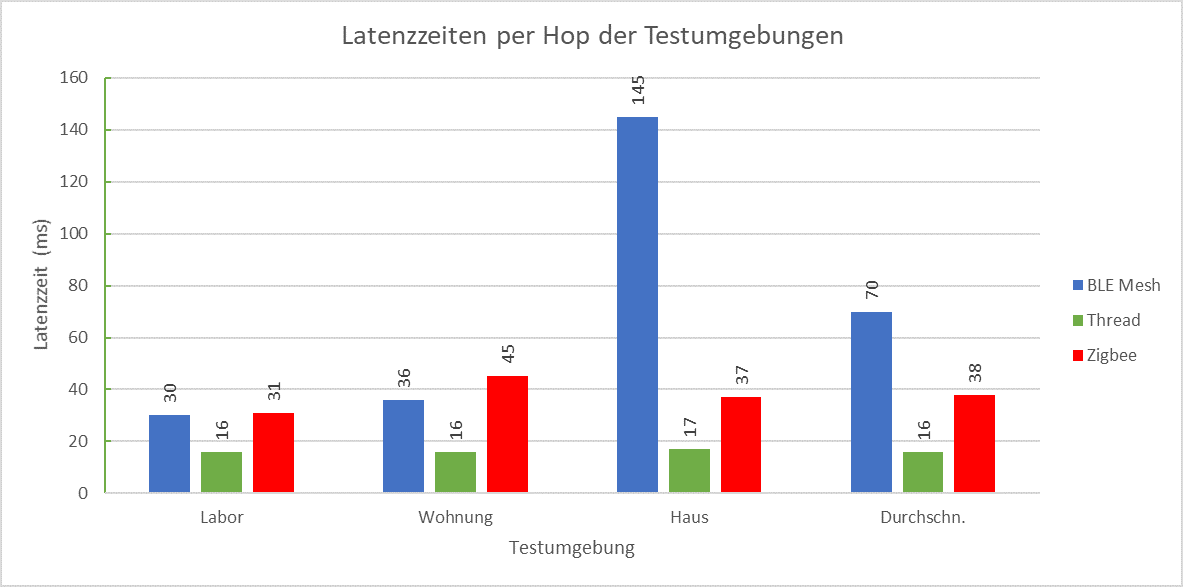
\includegraphics[width=1.0\textwidth]{Latenzzeiten_per_Hop_Testumgebungen.png}
	\caption{Durchschnittliche Latenzzeit per Hop der einzelnen Testumgebungen im Vergleich}\label{fig:Latenzzeiten_per_Hop_Testumgebungen}
\end{figure}

Die Abbildung \ref{fig:Latenzzeiten_per_Hop_Testumgebungen} zeigt das die Testumgebung Labor für alle Netzwerke die geringste Verzögerung aufweist. Bluetooth-Mesh erfährt bei weiter Streuung der Teilnehmer, wie sie im Haus anzutreffen ist, die grösste Steigerung der Latenz. Zigbee erhält in der Wohnung eine kaum relevante Erhöhung der Verzögerung. Thread zeichnet sich als unabhängig bezüglich der Testumgebung aus. 

\subsubsection{Durchsatz}\label{subsec:VergleichDurchsatzTestumgebungen}
\begin{figure}[H]
	\centering
	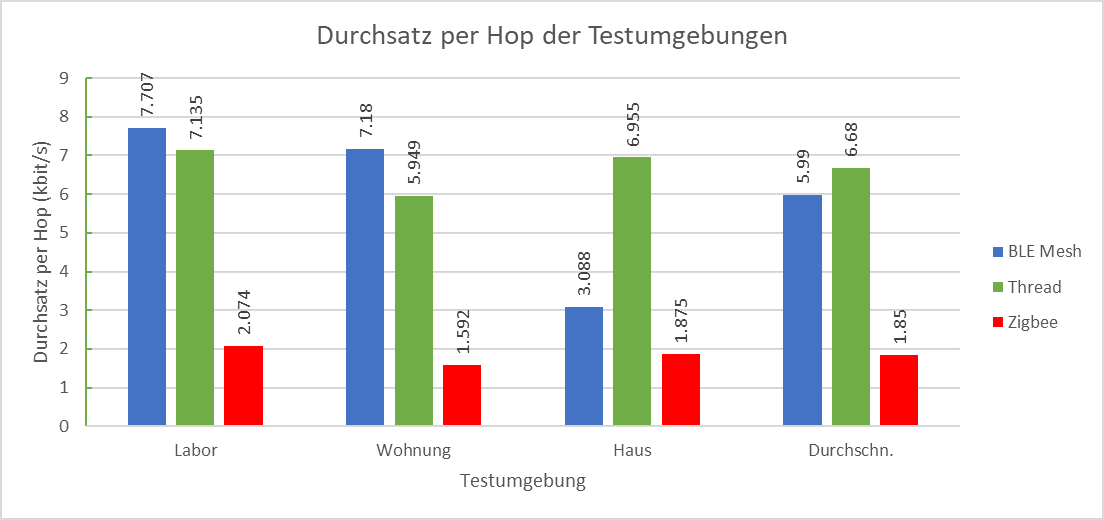
\includegraphics[width=1.0\textwidth]{Durchsatz_per_Hop_Testumgebungen.png}
	\caption{Durchschnittlicher Durchsatz per Hop der einzelnen Testumgebungen im Vergleich}\label{fig:Durchsätze_per_Hop_Testumgebungen}
\end{figure}

Ähnlich zu den Betrachtungen der Latenzzeit, zeigt die Abbildung \ref{fig:Durchsätze_per_Hop_Testumgebungen} den höchsten Durchsatz im Testaufbau Labor. Bluetooth-Mesh erfährt den grössten Einfluss durch ein ändern der Topologie. 

\subsubsection{Paketverlust}\label{subsec:VergleichPaketverlustTestumgebungen}
\begin{figure}[H]
	\centering
	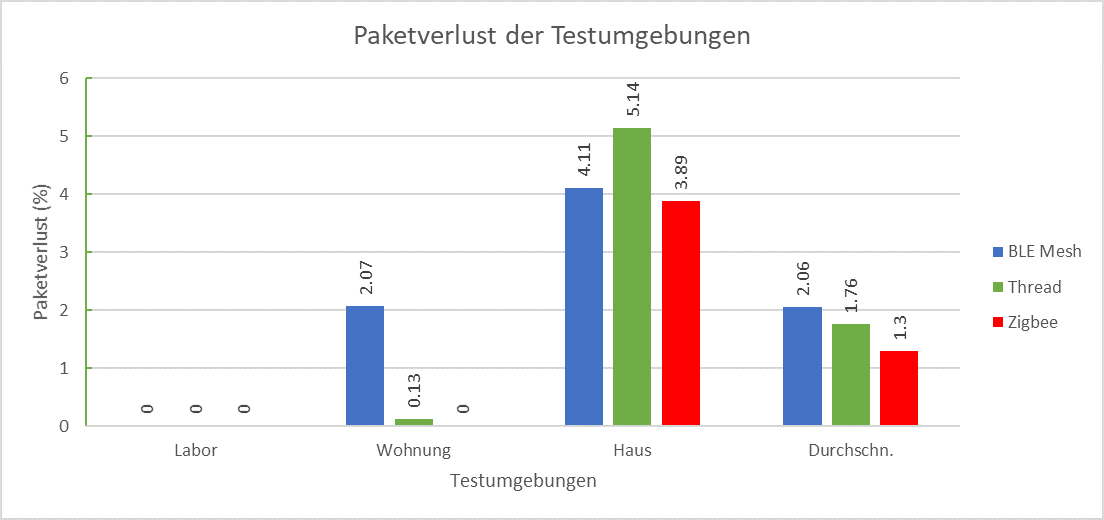
\includegraphics[width=1.0\textwidth]{Paketverlust_Testumgebungen.png}
	\caption{Durchschnittlicher Paketverlust der einzelnen Testumgebungen im Vergleich}\label{fig:PaketverlusteTestumgebungen}
\end{figure}

Abbildung \ref{fig:Durchsätze_per_Hop_Testumgebungen} zeigt das im Labor-Aufbau alle Netzwerke vollkommen zuverlässig arbeiten. In der Wohnung erlebt Bluetooth-Mesh einen geringen Anstieg des Paketverlusts. Bei Thread ist die Änderung kaum relevant. Alle Netzwerke erfahren bei starker Verzweigung des Netzwerks einen Anstieg der Verlustrate wie es bei der Haus-Topologie zu sehen ist. 

\subsection{Fazit}\label{subsec:FazitVergleich}
Die Ergebnisse aus den Messreihen 1 bis 4 aus allen Testumgebungen wurden als Durchschnittswert zusammengefasst, um einen finalen Vergleich zu erzielen. Abbildung \ref{fig:Messresultate_Fazit} zeigt alle Ergebnisse auf einen Blick. Thread geht shliesslich als klarer Sieger hervor. Dieser Netzwerk-Stack hat die Tests mit den besten Ergebnissen absolviert. Auf dem zweiten Platz steht Zigbee, welches mit seiner konstanten Latenz und als zuverlässigstes Protokoll die Daten verarbeiten konnte. Dabei gilt zu beachten, dass bei Zigbee die Anzahl Hops nicht berücksichtigt wurden (siehe Abschnitt \ref{sec:Validierung}), was zu einer leichten Verfälschung der Ergebnisse führt. Bluetooth-Mesh kann zwar durch den niedrigen Energiebedarf brillieren, schneidet jedoch in Sachen Performance deutlich schlechter ab als seine Konkurrenten Thread und Zigbee. Im Anschluss wird jedes Protokoll genauer analysiert und auf die Vor- und Nachteile sowie mögliche Verbesserungen eingegangen. 

\begin{figure}[H]
	\centering
	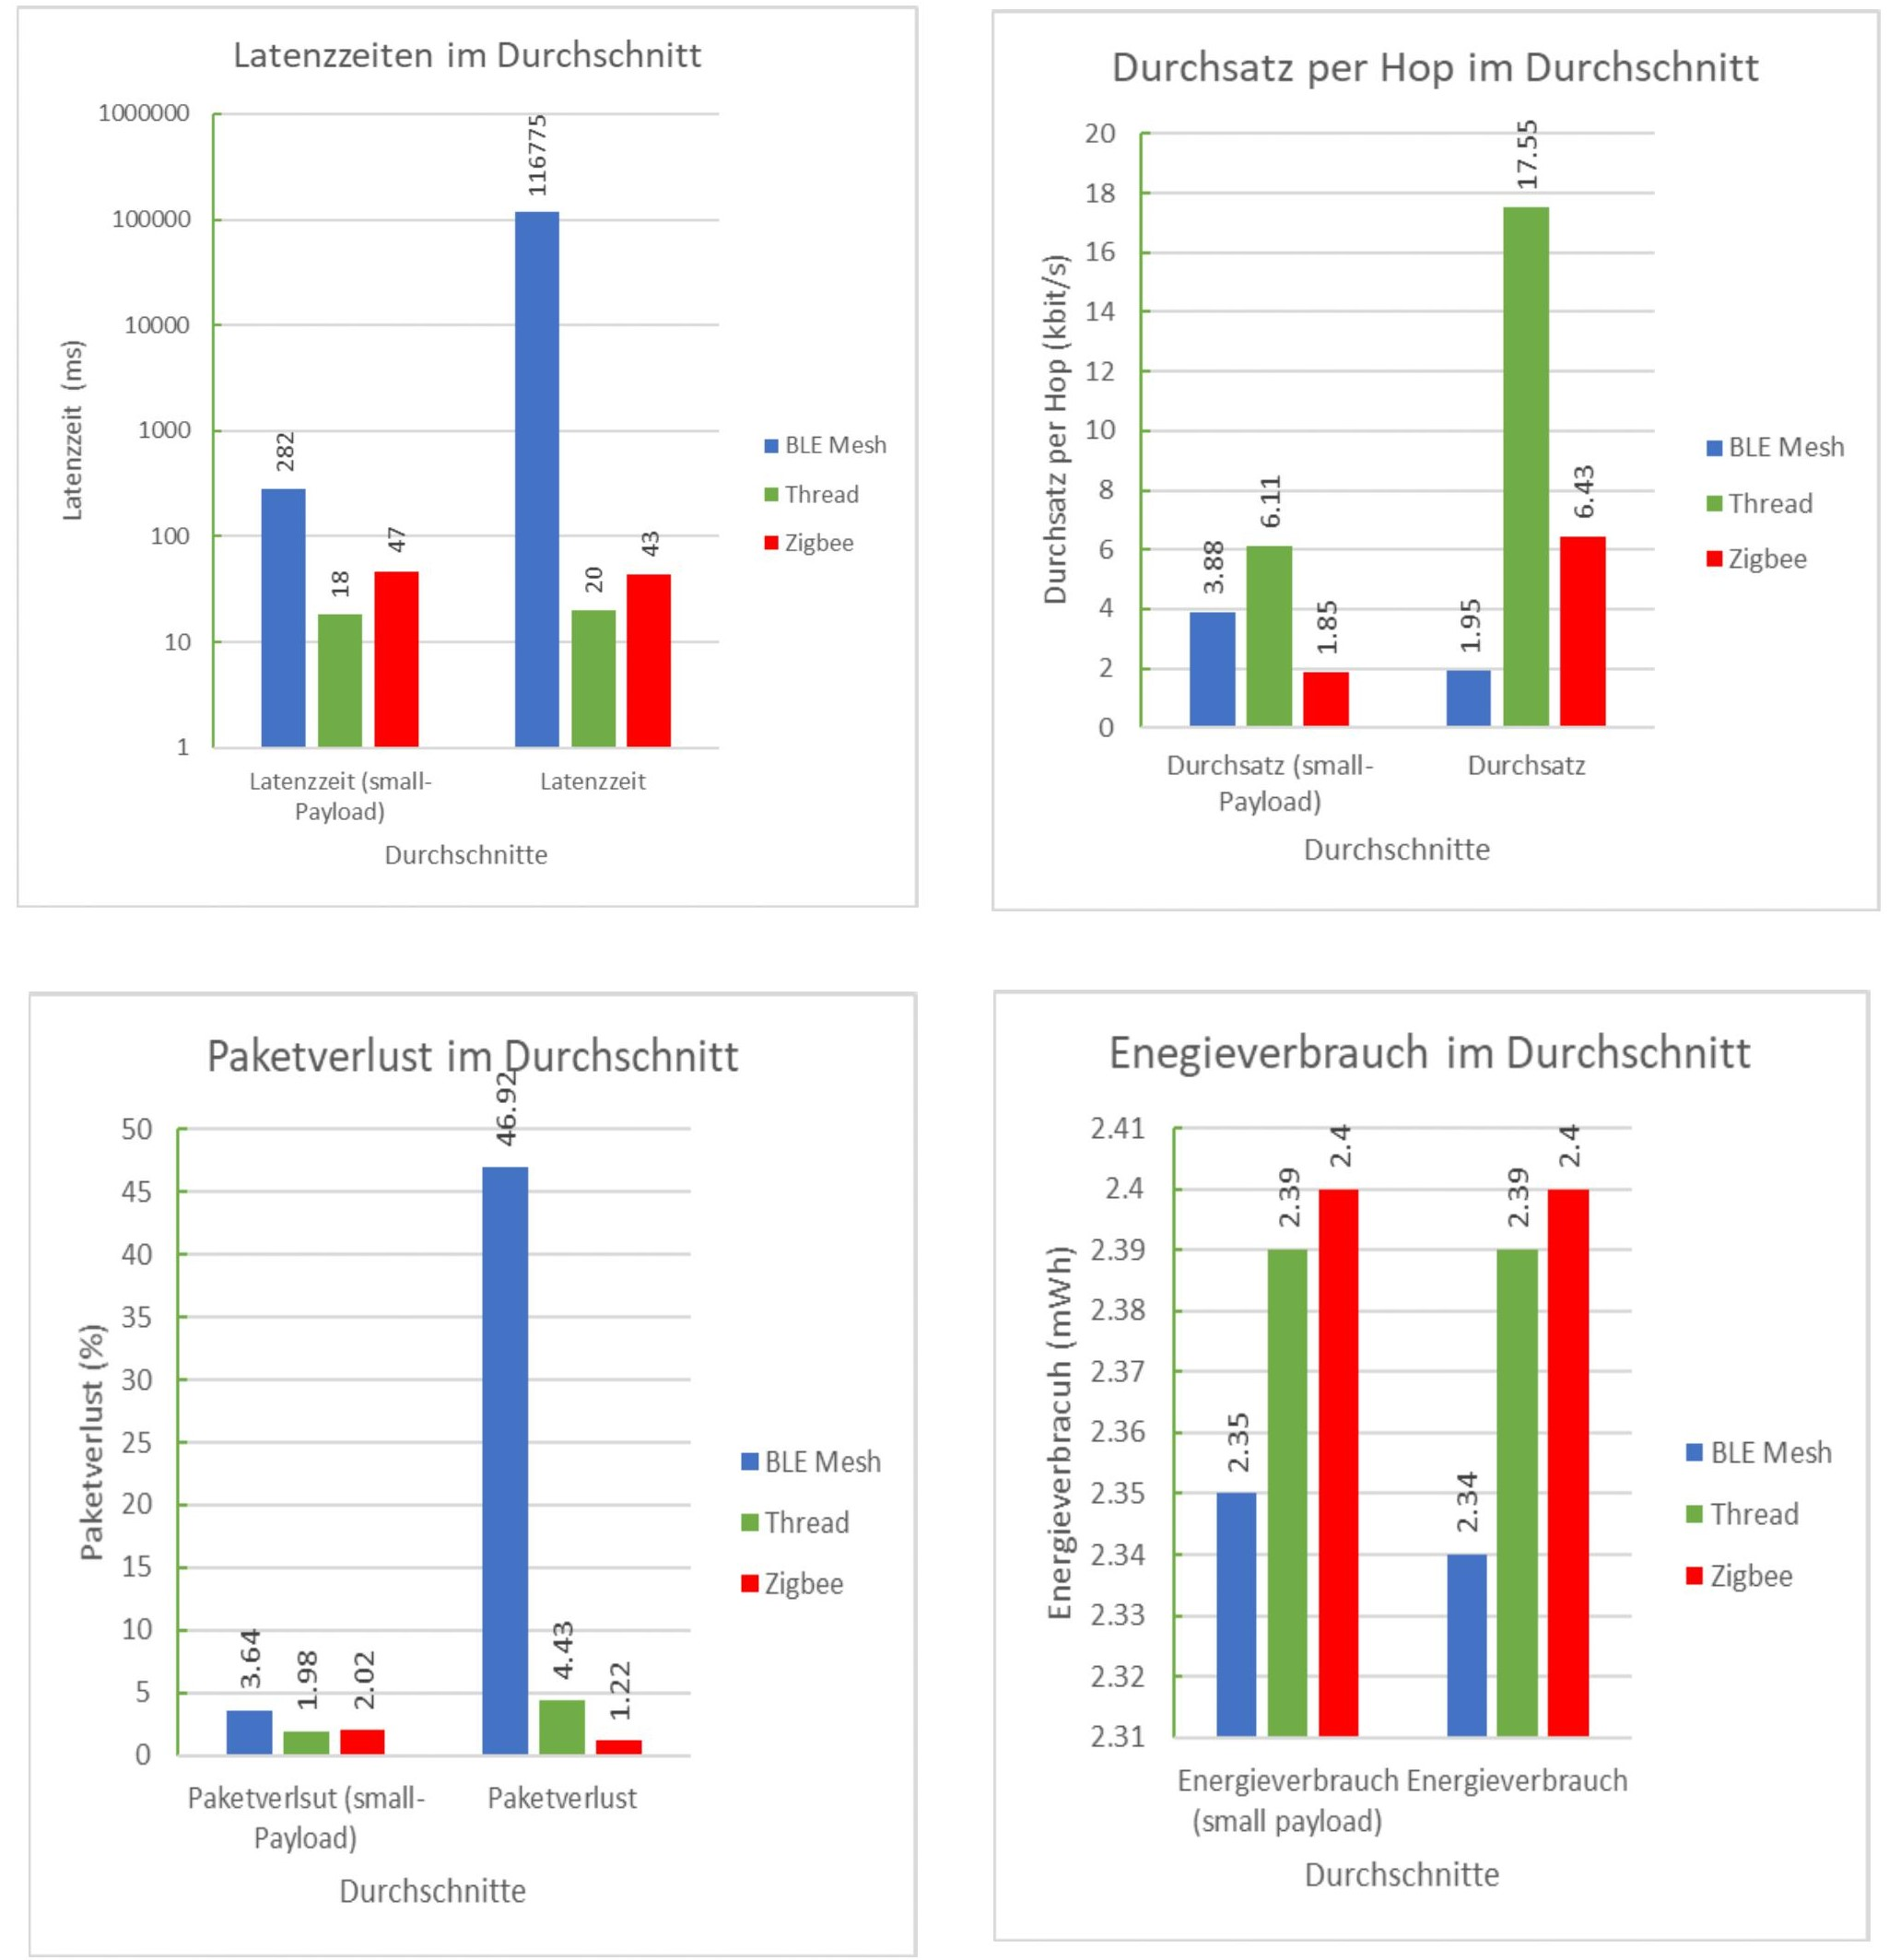
\includegraphics[width=1.0\textwidth]{Messresultate_Fazit.jpg}
	\caption{Durchschnittliche Messgrössen im Vergleich inkl. separater Betrachtung der Messergebnisse, welche mit 8-Byte Paketlänge erzielt wurden}\label{fig:Messresultate_Fazit}
\end{figure}

\subsubsection{Thread}\label{subsubsec:FazitThread}
Wie aus den vorhergehenden Kapiteln ersichtlich, hat der Thread Stack die Messungen mit den besten Ergebnissen abgeschlossen.
Das bedeutet aber nicht unbedingt, dass der Stack der Beste ist.
Es ist klar zu erkennen, dass der Thread Stack dank seiner automatischen Bestimmung von Routing-Knoten, sich seiner Umgebung gut anpassen kann.
Die Latenzzeit der gesendeten Nachrichten ändert sich in verschiedenen Umgebungen nur minimal.
Das bedeutet, dass sich der Thread Stack sehr gut für eine Hausautomation eignet.
Wenn sich Sensoren oder Aktoren verschieben, z.B. wenn eine Lampe einen neuen Standort erhält, erkennt dies der Stack und kann das Routing der Knoten anpassen.
Da sich das Netz sehr gut erweitern lässt und sich die Latenzzeiten eher tief zeigen, kann das Thread Netzwerk ausserdem gut für Industrieanwendungen verwendet werden. 

Durch das automatische Routen der Knoten entsteht auf den einzelnen Nodes jedoch ein Overhead, der zum Beispiel BT Mesh nicht aufweist.
Aus diesem Grund ist der Energieverbrauch auf den Knoten höher, was sich auch in der Energiemessung zeigt (Siehe Fachbericht). Dies ist zwar keine repräsentative Messung, da nur die aktiven Radio Zeiten gemessen wurden. Dennoch kann es die vorherige These mit dem Overhead bestätigen. 

Anders als bei BT-Mesh können mit dem IEEE 802.15.4 und dem 6LoWPAN Layer grössere Pakete versendet werden. Das bedeutet, dass die Segmentierung im Gegensatz zu BT Mesh später stattfindet. Dies erklärt das Phänomen, dass sich der Durchsatz mit steigender Payload vergrössert. Der Thread Stack erreicht bei manchen Messreihen einen Durchsatz von bis zu 32 kbit pro Sekunde. Dies ist jedoch eher unwahrscheinlich. Da bei den Durchschnittsberechnungen kein Median verwendet wurde, können Extremwerte den Durchschnitt verfälschen. Es gab sehr wenige Latenzmessungen, die fehlerhaft waren und eine Latenz unter 0.5ms aufwiesen. Durch diesen Fehler wurde der Durchsatz in der Auswertung unwahrscheinlich hoch. 

\subsubsection{Zigbee}\label{subsubsec:FazitZigbee}
Die Resultate und Vergleiche aus den vorhergehenden Abschnitten zeigen, dass das Zigbee Protokoll in dieser Implementation eine solide Performance abliefert.
Auch wenn Zigbee nicht ganz an jene Leistung von Thread herankommt, zeigen die Ergebnisse wieso Zigbee zurzeit das am weitest verbreitete WPAN Protokoll ist.

Die durchschnittlichen Latenzzeiten liegen zwischen 30ms und 50ms. Damit schneidet Zigbee besser als Bluetooth ab, jedoch liegen die Ergebnisse hinter jenen Durchschnittswerten von Thread.
Dies kommt nicht allzu überraschend.
Sehr interessant zu beobachten sind die Verteilungen der Latenzzeiten, wie sie beispielsweise in Abbildung \ref{fig:VerteilungderLatenzzeiten} zu sehen sind.
Anders als Thread weist Zigbee dort deutliche Peaks bei 40ms und 70ms auf.
Diese Beobachtung kann bei sämtlichen Messresultaten gemacht werden.
Ausreisser nach unten gibt es praktisch keine und solche nach oben nur sehr vereinzelt.
Es kann also festgestellt werden, dass bei Zigbee mit einer minimalen Latenzzeit von ca. 30ms gerechnet werden muss, diese Schwelle aber in den seltensten Fällen deutlich überschritten wird.
Zigbee wäre also auch für eher zeitkritische Anwendungen geeignet, da die Latenzzeiten deterministisch sind.
In diesen Zusammenhang nochmals zu erwähnen ist, dass die Information über die Anzahl Hops die ein Paket passiert hat, leider nicht erfasst werden konnte.
Es kann davon ausgegangen werden, dass der Peak bei 70ms in den Latenzzeiten, diesem Problem verschuldet ist.
Wenn also die Anzahl Hops erfasst werden könnten, dürfte sich die Verteilung der Latenzzeiten wohl nochmals reduzieren und die Ergebnisse würden noch besser ausfallen.

Die Ergebnisse aus Abbildung \ref{fig:Latenzzeiten_per_Hop_Messreihen} zeigen eine weitere interessante Eigenschaft von Zigbee.
In Messreihe 1 beträgt die durchschnittliche Latenzzeit von 86ms mehr als das Doppelte der Durchschnittswerte in den übrigen Messreihen.
Die Ursache dafür kann nicht abschliessend geklärt werden.
Jedoch liegt die Vermutung nahe, dass sich das Mesh Netz während dieser Messreihe noch nicht komplett aufgebaut respektive das \textit{Commissioning} und \textit{Route Discovery} noch nicht abgeschlossen war.
Dies verursachte zusätzlichen Traffic und beeinflusste den Benchmark.

Auffallend tief ist auch der Paketverlust.
In den meisten Fällen lag dieser sogar bei 0 Prozent.
Hier macht sich das CSMA\slash CA des \textit{IEEE 802.15.4} MAC Layers bemerkbar.
Zudem wirkt sich hier wohl die Unicast Adressierung innerhalb von Zigbee positiv aus.
Die Gesamtbelastung des Netzes kann dadurch deutlich minimiert werden.

Die Erhöhung der Payload von 8 auf 50 Byte hat die Latenzzeiten bei den Zigbee Messungen nicht merklich beeinflusst.
Dies bewirkt, dass der Durchsatz mit grösserer Payload zunimmt.
Da die Segmentierung dank \textit{IEEE 802.15.4} erst ab 127 Byte Framelänge startet, ist dies auch nicht weiter verwunderlich.
Gegenüber BT-Mesh haben Zigbee wie auch Thread den klaren Vorteil grössere Payloads versenden zu können, ohne segmentieren zu müssen.

Zigbee brilliert in den Anwendungen, in denen es bereits verbreitet eingesetzt wird.
Beispielsweise eine komplette Hausautomation oder eine einfachere Lichtsteuerung.
Bis zu einer Netzwerkgrösse von ungefähr 200 Nodes mit einigermassen kleinem Verkehrsaufkommen ist Zigbee die ideale Wahl.
Ergänzt durch die \textit{Zigbee Cluster Library} welche die Systeme herstellerunabhängig macht wird Zigbee noch interessanter.


\subsubsection{Bluetooth Mesh}\label{subsubsec:FazitBluetoothMesh}
Die Performance von Bluetooth-Mesh ist stark von der Belastung abhängig.
Der grösste Einfluss auf die Performance hatte die Länge der gesendeten Nachrichten.
Ursache dafür ist, dass ein einzelnes Bluetooth-Mesh-Paket lediglich 10-Byte Payload aufnehmen kann. Der Stack beginnt mit der Segmentierung der Daten in mehrere kleine Pakete. Bei 32-Byte sind dies bereits 4 Frames. Damit ist der Network-Stack überfordert. 

\begin{figure}[H]
	\centering
	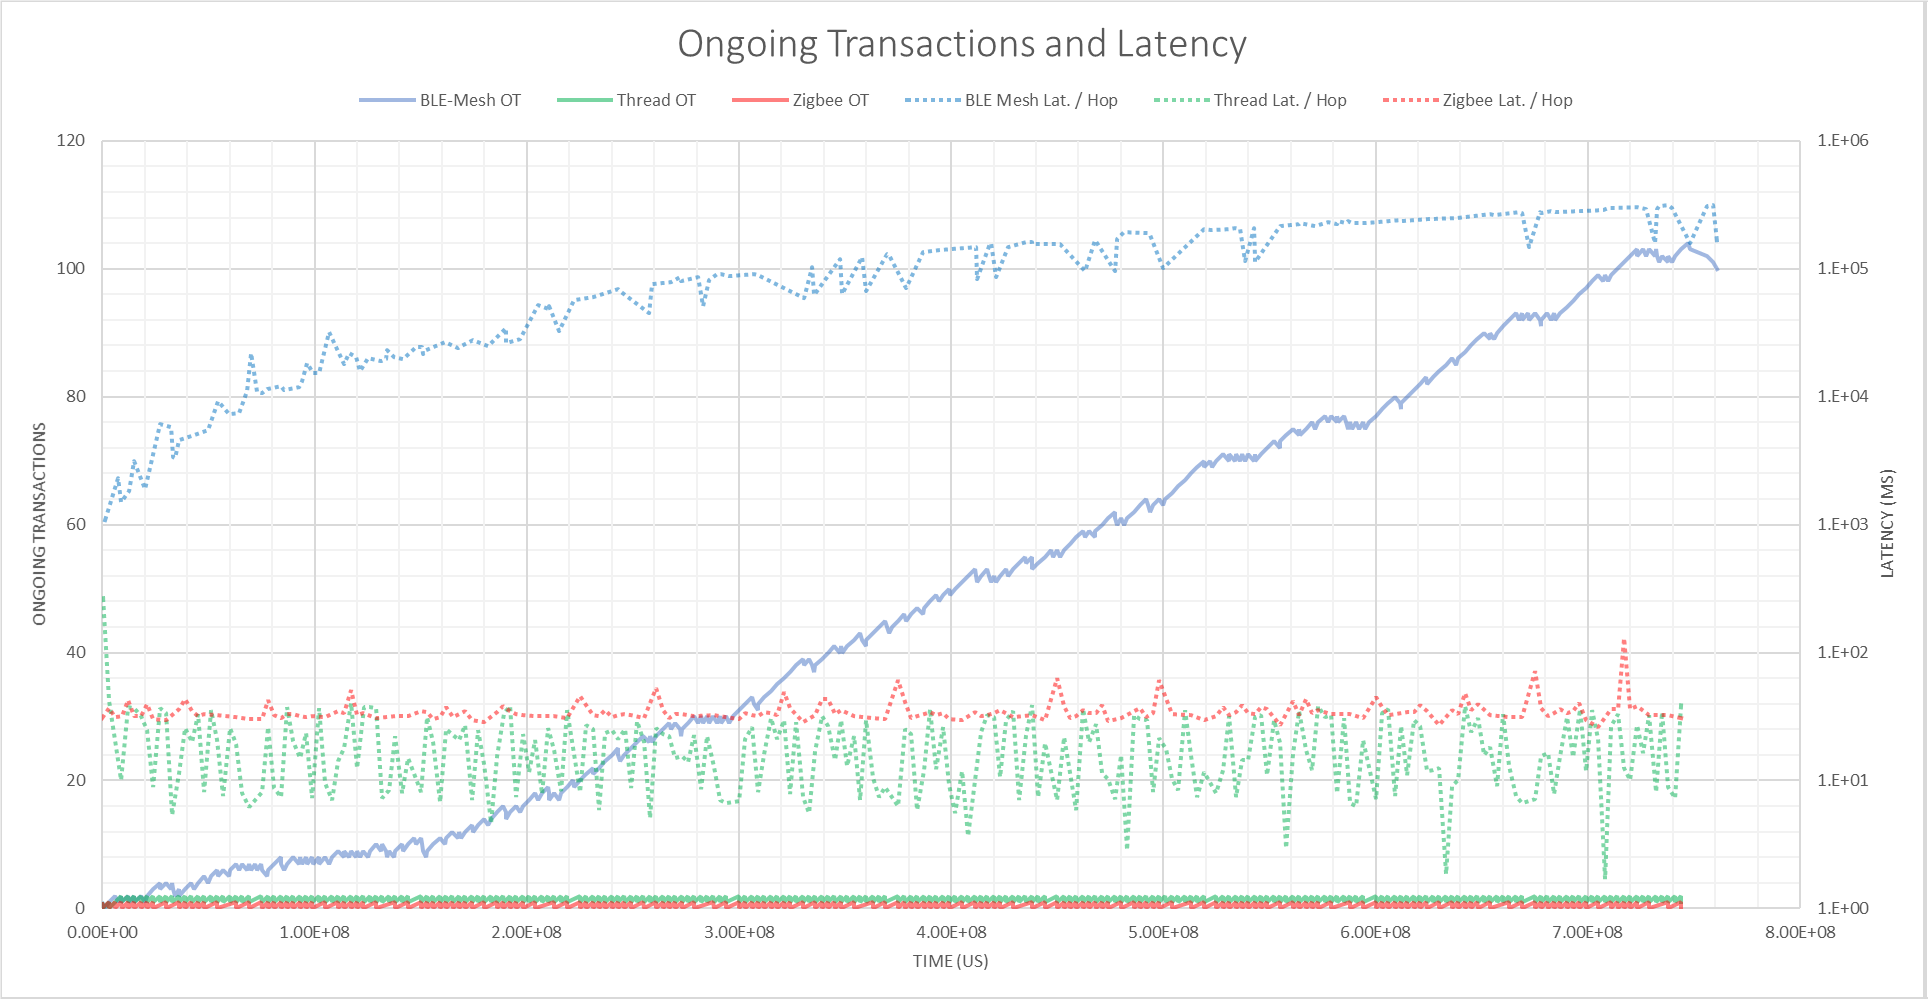
\includegraphics[width=0.7\textwidth]{Bluetooth_Mesh_Big_Payload_Issue.png}
	\caption{Ongoing Transactions und Latenzzeiten einer Messung mit 32Byte Paketlänge}\label{fig:Bluetooth_Mesh_Big_Payload_Issue}
\end{figure}
\vspace{-5mm}
Abbildung \ref{fig:Bluetooth_Mesh_Big_Payload_Issue} zeigt eine Messung mit 32-Byte Payload bei einer Message-Dichte von 3 Sekunden/Message, welche sequentiell versendet wurden.
Dabei ist zu erkennen, dass die Anzahl der Ongoing Transactions immer weiter ansteigt.
Erst in der Nachtbearbeitungszeit sinkt die Kurve wieder.
Dies deutet darauf hin, dass zu viel Traffic im Netz vorhanden ist. In Korrelation mit den Ongoing Transactions steigt die Latenz von einer Sekunde auf einige 100 Sekunden an. Vermutlich entsteht eine zu hohe Message-Dichte, da zu viele Relay-Nodes die empfangenen Messages wiederholen. Durch deaktivieren einiger Relays könnte der Netzaufbau entlastet werden. Jedoch erfordern solche manuellen Eingriffe Fachwissen und verringern die Ausfallsicherheit des Netzes. 
\pagebreak

\clearpage
\section{Validierung und Verifizierung}\label{sec:ValidierungVerifizierung}

\subsection{Validierung}\label{subsec:Validierung}
Die durchgeführten Messungen haben aussagekräftige Resultate geliefert welche jedoch stark vom gewählten Vorgehen abhängig sind.
Dieses Vorgehen soll nun kritisch überprüft und allfällige Mängel im Konzept sowie der Umsetzung aufgezeigt werden.
Zudem werden systematische Messfehler deklariert.

\paragraph{Large Payload}
Die Messungen 3, 4 und 8 gemäss Tabelle \ref{tab:MessungenMeshBenchmark} welche mit einer grossen Payload durchgeführt wurden, sind nur für Thread und Zigbee aussagekräftig. Der BT Mesh Stack liefert bei diesen Messungen keine brauchbaren Resultate.
Eine Recherche zu diesem Problem hat ergeben, dass durch die Fragmentierung einer 32 Byte Payload die sichere und schnelle Übertragung der Daten nicht mehr gewährleistet werden kann.

\paragraph{Zigbee Latency}
Wie bereits im Abschnitt \ref{subsec:Resultate} erwähnt, konnte bei Zigbee die Anzahl Hops die ein Paket passiert hat nicht ausgewertet werden.
Der Forumsbeitrag \href{https://devzone.nordicsemi.com/f/nordic-q-a/63815/zigbee---read-number-of-hops-radius}{\textit{Zigbee - Read number of hops (radius)\footnote{\url{https://devzone.nordicsemi.com/f/nordic-q-a/63815/zigbee---read-number-of-hops-radius}}}} bestätigt, dass der entsprechende Wert mit der verwendeten SDK nicht ausgelesen werden kann.
Als Folge dessen kann schliesslich die Latenzzeit nur als Total über die gesamte Strecke erfasst werden. In der Auswertung verschafft dies BT Mesh und Thread fälschlicherweise einen Vorteil gegenüber Zigbee.
Die Auswertung der totalen Latenzzeit bei allen 3 Protokollen könnte das Problem lösen.
Dies würde jedoch dem Messkonzept widersprechen und wurde deshalb nicht für alle Messungen umgesetzt.
Die Abbildungen \ref{fig:DurchschnittlicheLatenzzeitValidierung} und \ref{fig:DurchschnittlicheLatenzzeitohneHopsValidierung} zeigen den Unterschied am Beispiel der oben analysierten Messung \ref{subsec:Resultate}.
Während links die Latenzzeit pro Hop dargestellt ist, zeigt die rechte Grafik die totale Latenzzeit.
Der Unterschied ist vorallem bei Thread deutlich erkennbar.
Bereits in der Abbildung \ref{fig:VerteilungderLatenzzeiten} ist das Problem zu erkennen.
Die Statistik der Latenzzeiten von Zigbee hat zwei Hauptsäulen bei 40ms und 70ms was auf einen Hop hindeutet.


\begin{figure}[!htbp]
	\centering
	\begin{minipage}[b]{0.49\textwidth}
		\centering
		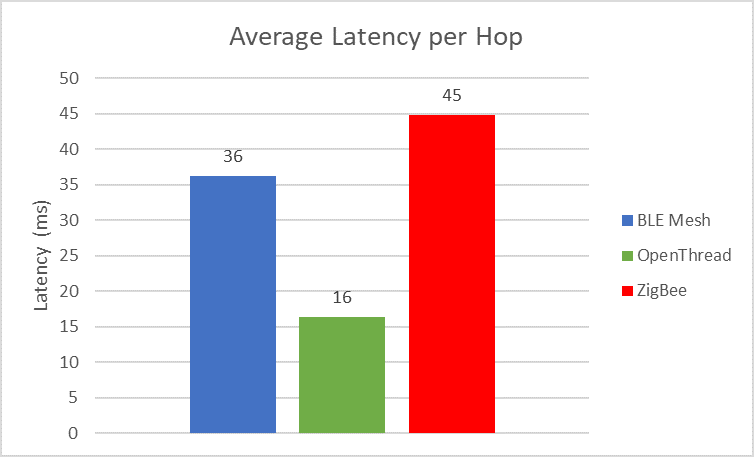
\includegraphics[width=\textwidth]{Average_Latency_per_Hop.png}
		\caption{Durchschnittliche Latenzzeit pro Hop}
		\label{fig:DurchschnittlicheLatenzzeitValidierung}
	\end{minipage}
	\begin{minipage}[b]{0.49\textwidth}
		\centering
		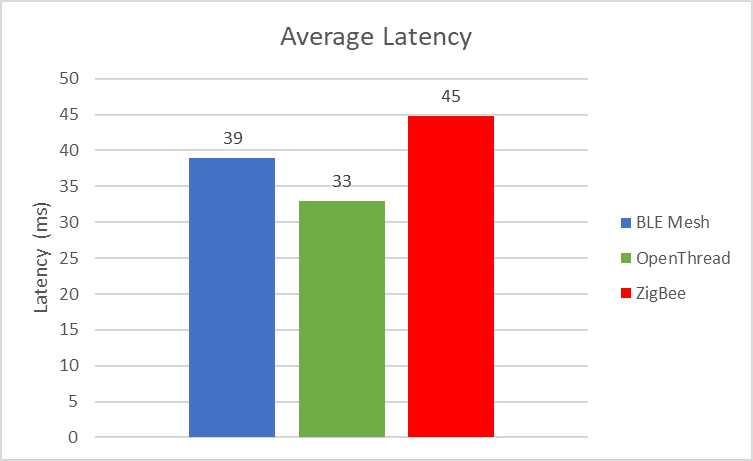
\includegraphics[width=\textwidth]{Average_Latency_without_Hops.png}
		\caption{Durchschnittliche Latenzzeit ohne Berücksichtigung der Hops.}	\label{fig:DurchschnittlicheLatenzzeitohneHopsValidierung}
	\end{minipage}
\end{figure}

\newpage
\paragraph{Nachrichten Dichte}
Bei der Definition der Messreihen \ref{sec:Interpretation} wurden zu Beginn nur die Messungen 1 bis 6 spezifiziert.
Die Messreihen 7 und 8 kamen erst nachträglich hinzu als festgestellt werden musste, dass die Dichte der Nachrichten für den BT Mesh Stack zu hoch gewählt wurde.
Dieser schien überfordert besonders bei zufälliger Nachrichten Generierung.
Thread und Zigbee zeigten indes keine Mühe mit der Dichte von 60 Nachrichten in 600 Sekunden pro Node.
Die Resultate der Messungen 7 und 8 haben schliesslich gezeigt, dass die Reduktion der Nachrichtendichte einen positiven Einfluss hat.

\paragraph{Group addressing mode}
Der \textit{Group addressing mode} wurde für die 3 Protokolle unterschiedlich definiert.
Erste Tests vor den eigentlichen Benchmarks haben gezeigt, dass eine Multicast Adressierung bei Zigbee unbrauchbar ist.
Deshalb hat man sich entschieden bei Zigbee eine Unicast Adressierung umzusetzen.
Während den Benchmarks musste schliesslich festgestellt werden, dass Zigbee durch diese Änderung ein deutlicher Vorteil erlangt hat.
Besonders auf die Paketverlustrate hat sich die Unicast Adressierung positiv ausgewirkt denn Unicast Nachrichten werden im IEEE 802.15.4 Standard auf MAC Ebene quittiert.
Multicast resp. Broadcast hingegen nicht.

Auch in der Messung Nr. 5 hätte sich die Unicast Adressierung für Zigbee positiv ausgewirkt da die Netzbelastung deutlich geringer gewesen wäre.

\paragraph{Durchschnittswerte in den Resultaten}
In den Resultaten \ref{subsec:Resultate} wurden sämtliche Durchschnittswerte als Mittelwerte einschliesslich allfälliger Ausreisser aus den Messwerten gebildet.
Dadurch wurden gewisse Resultate deutlich verfälscht.
In einer neuen Auswertung müsste die Ursache für die einzelnen Ausreisser genauer geklärt werden und diese allenfalls gestrichen werden.


\subsection{Verifizierung}\label{subsec:Verifizierung}
Eine Verifizierung der Messresultate konnte nur anhand des Referenzberichts \textit{AN1142: Mesh Network Performance
	Comparison\footnote{\url{https://www.silabs.com/documents/public/application-notes/an1142-mesh-network-performance-comparison.pdf} \cite{silicon_laboratories_inc_an1142_2020}}} von \textit{Silicon Labs} gemacht werden.
Dieser ist auf der Webseite von \textit{Silicon Labs} einsehbar.

Der Vergleich der Messergebnisse hat gezeigt, dass die Grössenordnung der Resultate mit jenen aus dem Bericht von Silicon Labs übereinstimmt.
Selbst die Ausreisser in der Latenzzeit bei BT Mesh liegen im selben Rahmen.
Zudem kann die klare Abhängigkeit der Resultate von der Grösse der Payload bestätigt werden.
Einige Unterschiede sind jedoch in der Verteilung der Latenzzeiten erkennbar.
Im Referenzbericht ist diese in einem Bereich zwischen 20ms und 60ms ziemlich regelmässig während in den Ergebnissen dieser Thesis die Verteilung unregelmässiger daherkommt.
\pagebreak

\clearpage
%%---BIBLIOGRAPHY------------------------------------------------------------------------
{\sloppypar
\printbibliography[heading=bibintoc]
\label{sec:lit}
%\selectlanguage{ngerman}				%ngerman or english
%\printbibliography
}

%%---List of Figures------------------------------------------------------------------------
\listoffigures

%%---APPENDIX----------------------------------------------------------------------------
\begin{appendix} 

\addcontentsline{toc}{section}{Anhang}


%**********************Aufgabenstellung***************************
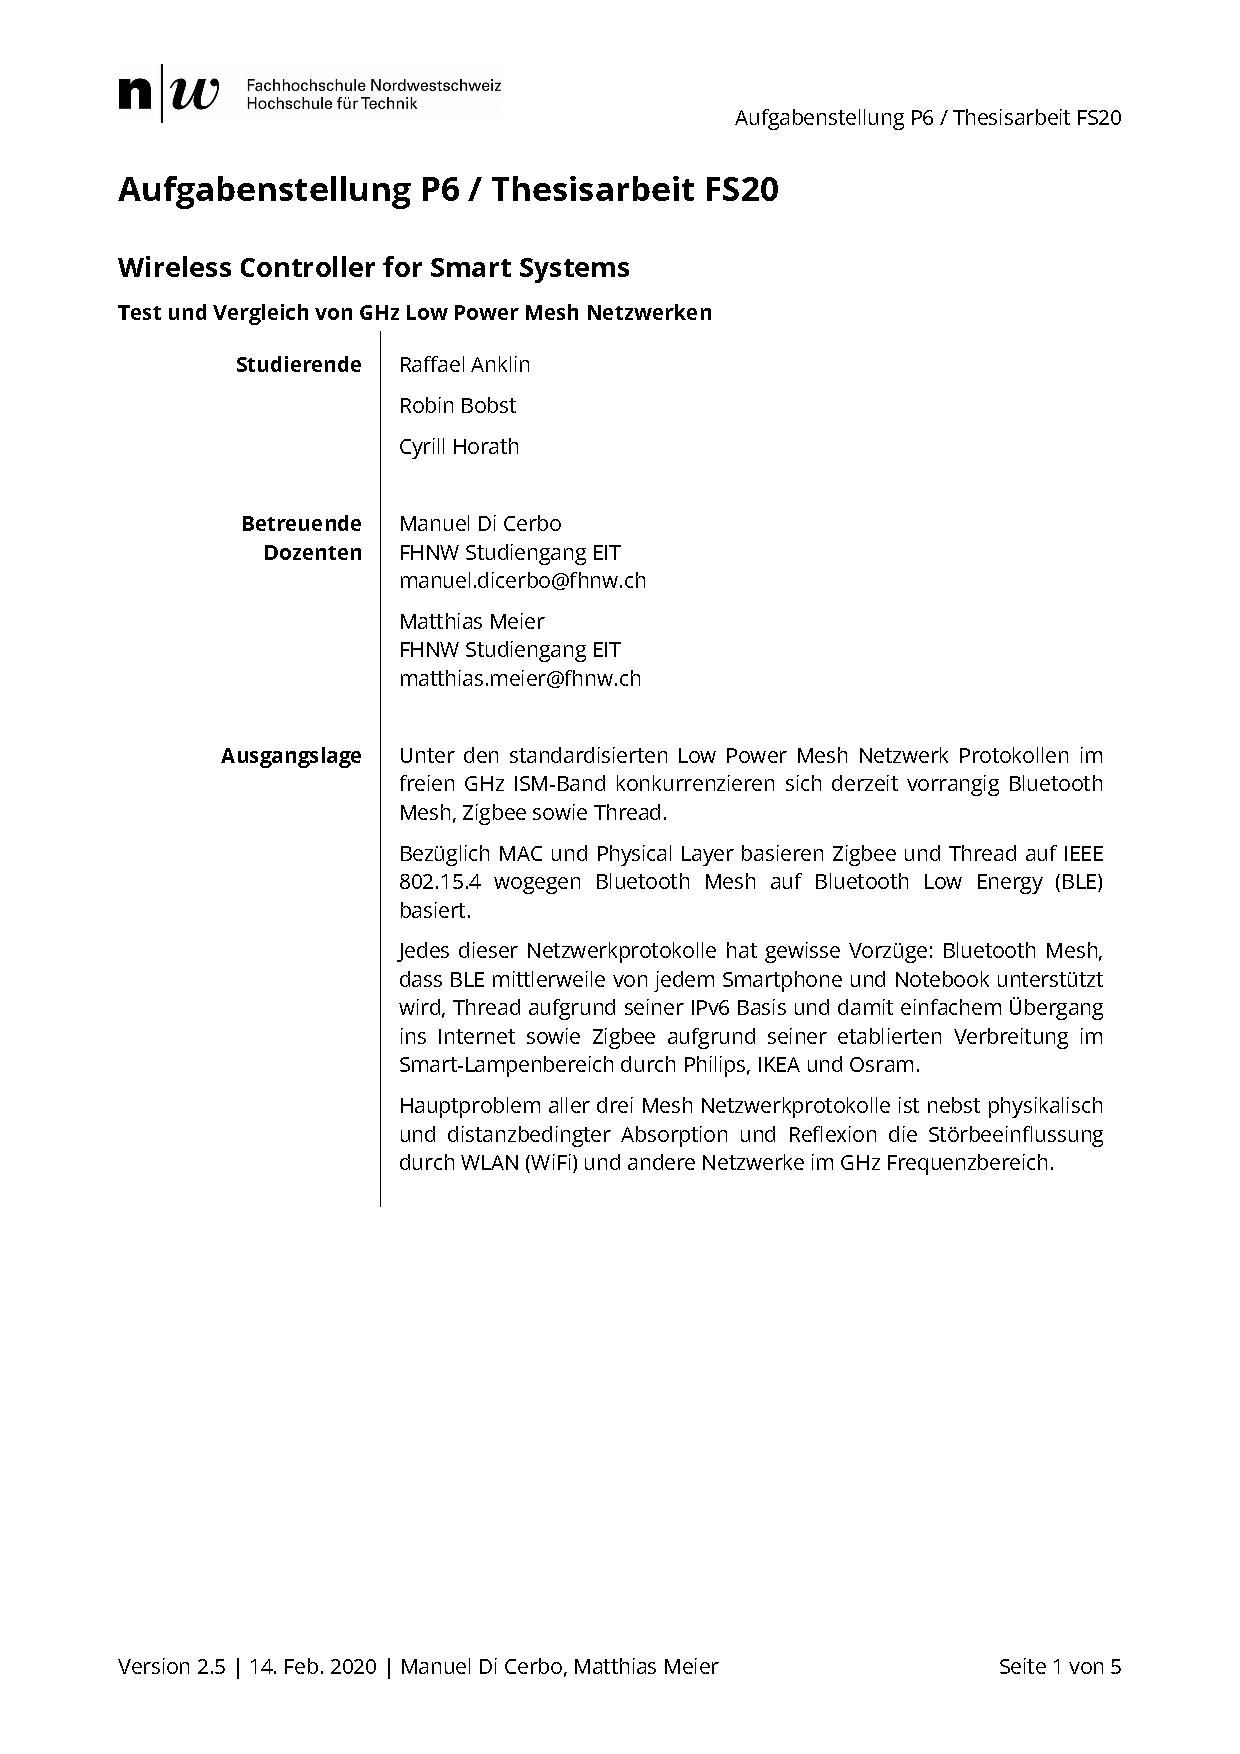
\includepdf[pages={1}, nup=1x1, landscape=false, scale=0.9 ,offset=0 -45, pagecommand={\section{Aufgabenstellung}\label{app:Aufgabenstellung}\thispagestyle{myheadings}}]{appendix/P6_Aufgabenstellung_Wireless_Controller_for_Smart_Systems.pdf}

\includepdf[pages={2-5}, nup=1x1, landscape=false, scale=0.9 ,offset=0 -45, pagecommand={\thispagestyle{myheadings}}]{appendix/P6_Aufgabenstellung_Wireless_Controller_for_Smart_Systems.pdf}


%**********************Pflichtenheft***************************
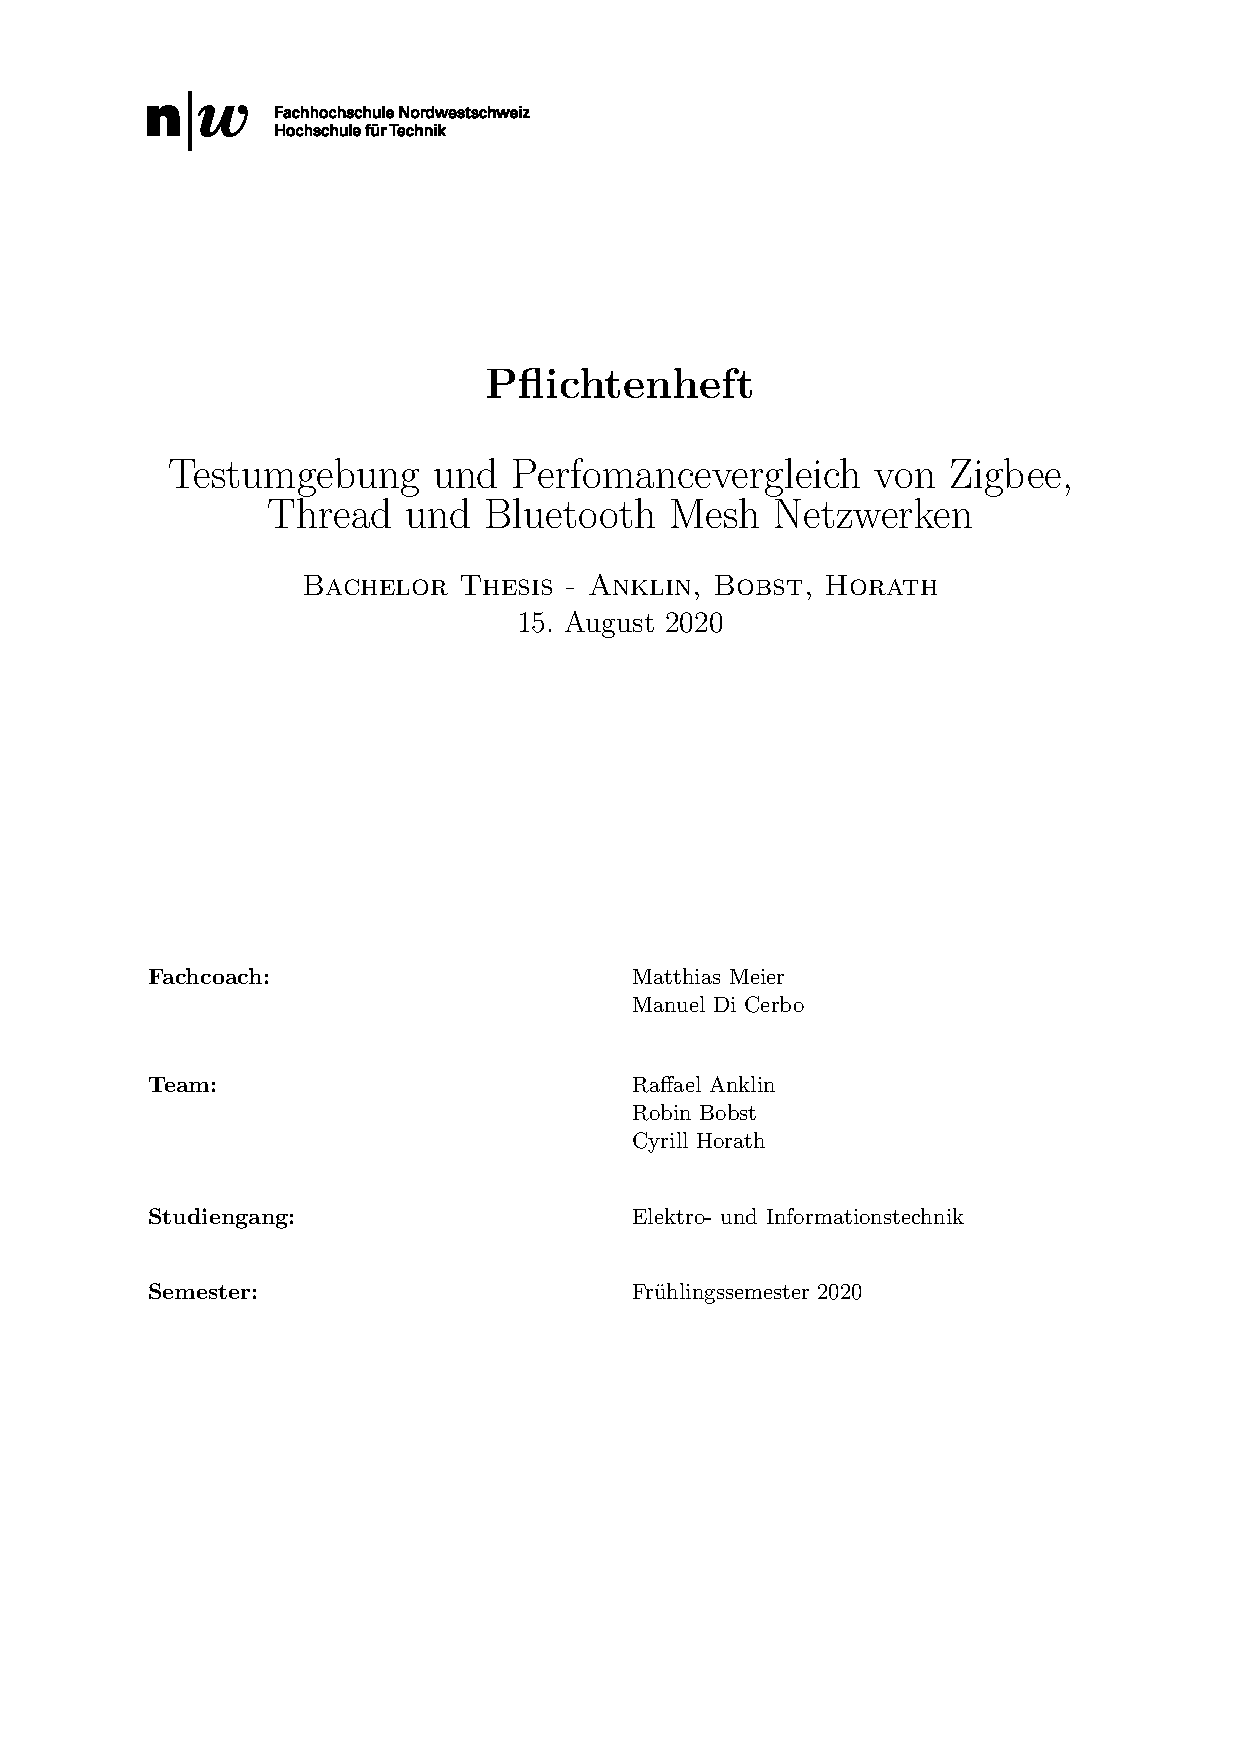
\includepdf[pages={1}, nup=1x1, landscape=false, scale=0.95 ,offset=0 -45, pagecommand={\section{Pflichtenheft}\label{app:Pflichtenheft}\thispagestyle{myheadings}}]{appendix/P6_Pflichtenheft.pdf}

\includepdf[pages={2-19}, nup=1x1, landscape=false, scale=0.95 ,offset=0 -45, pagecommand={\thispagestyle{myheadings}}]{appendix/P6_Pflichtenheft.pdf}

%***************EMV Bericht Abstrahlung Antennen*********************
\includepdf[pages={1}, nup=1x1, landscape=false, scale=0.95 ,offset=0 -45, pagecommand={\section{Bericht emv Messung Development Kits}\label{app:BerichtemvMessungDevelopmentKits}\thispagestyle{myheadings}}]{appendix/emv_Bericht_FS20.pdf}

\includepdf[pages={2-13}, nup=1x1, landscape=false, scale=0.95 ,offset=0 0, pagecommand={\thispagestyle{myheadings}}]{appendix/emv_Bericht_FS20.pdf}

%***************Messprotokolle Mesh Benchmark*********************
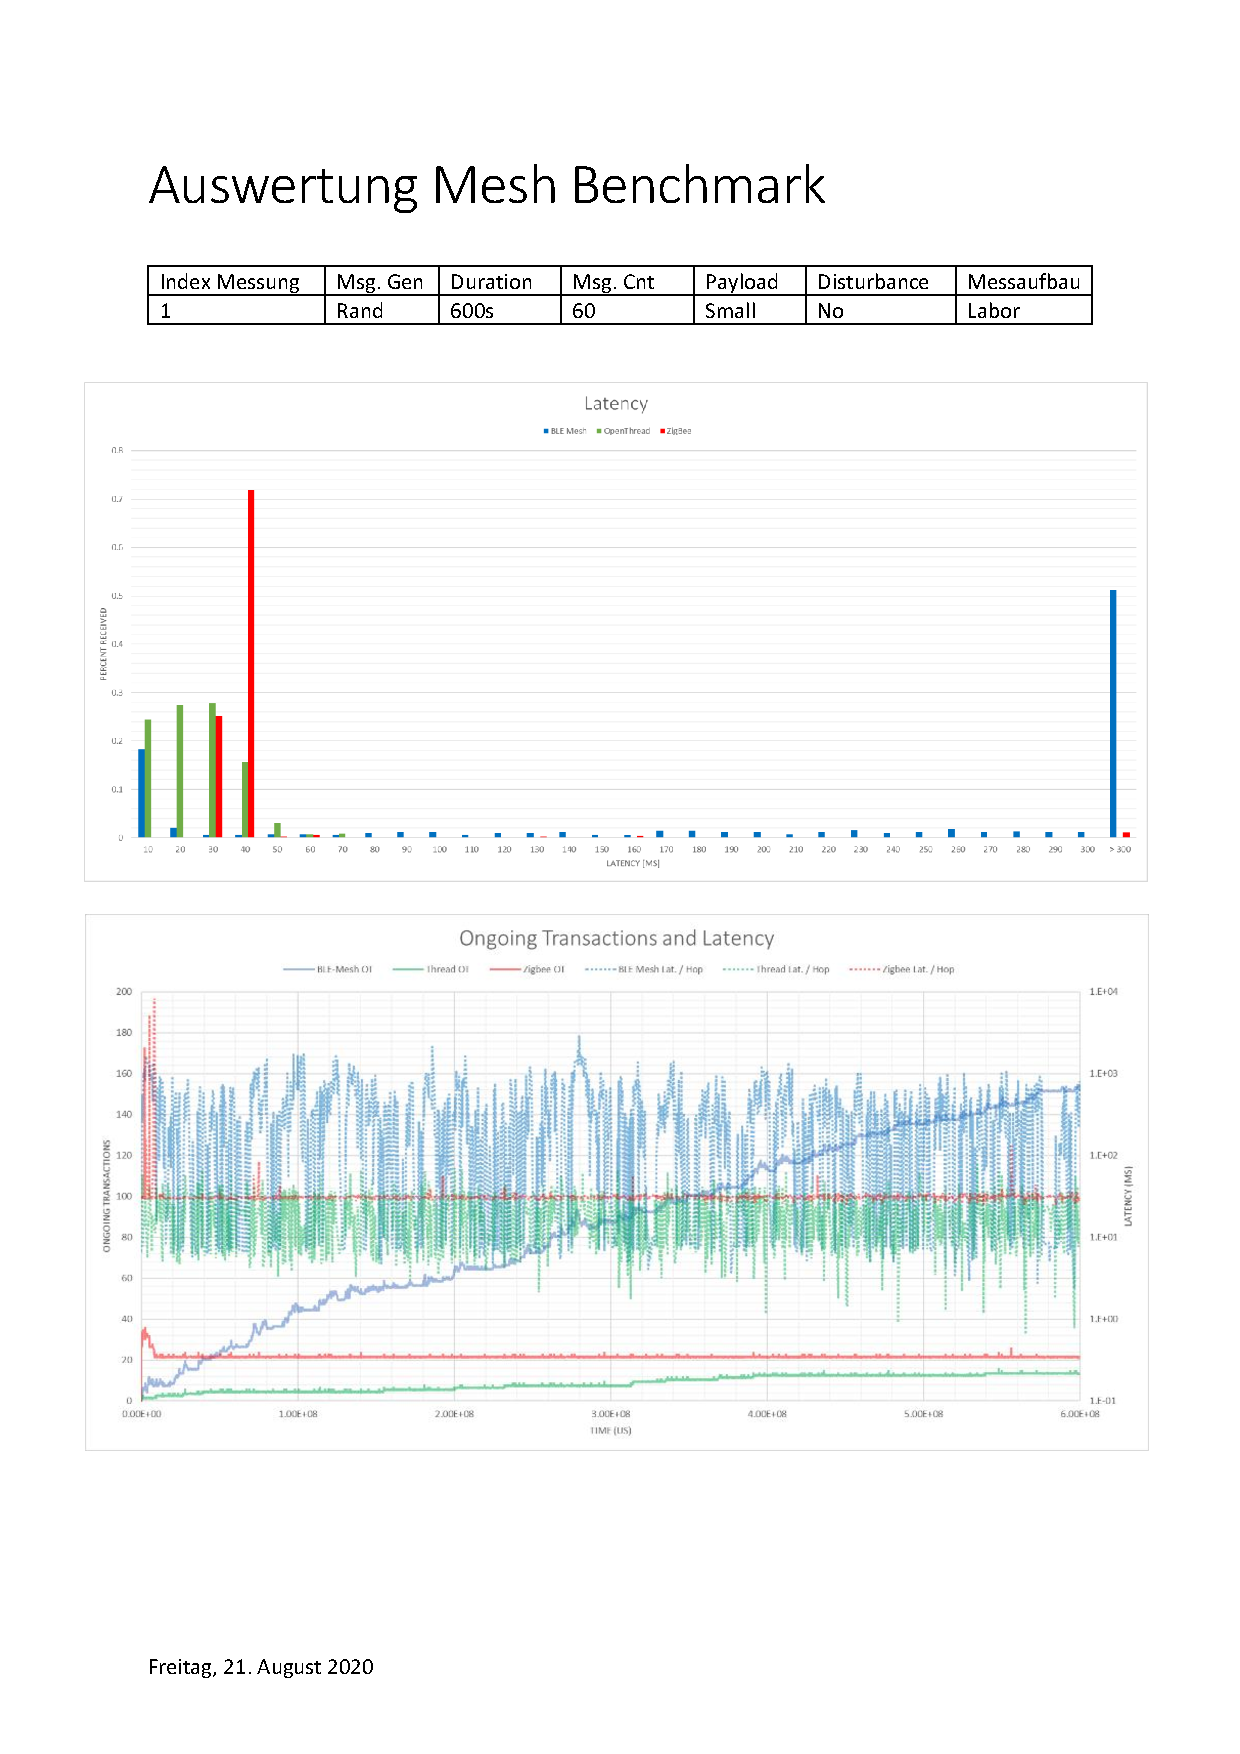
\includepdf[pages={1}, nup=1x1, landscape=false, scale=0.95 ,offset=0 -20, pagecommand={\section{Messprotokolle Mesh Benchmark}\label{app:MessprotokolleMeshBenchmark}\thispagestyle{myheadings}}]{appendix/Messprotokolle_Labor.pdf}

\includepdf[pages={2-14}, nup=1x1, landscape=false, scale=0.95 ,offset=0 0, pagecommand={\thispagestyle{myheadings}}]{appendix/Messprotokolle_Labor.pdf}

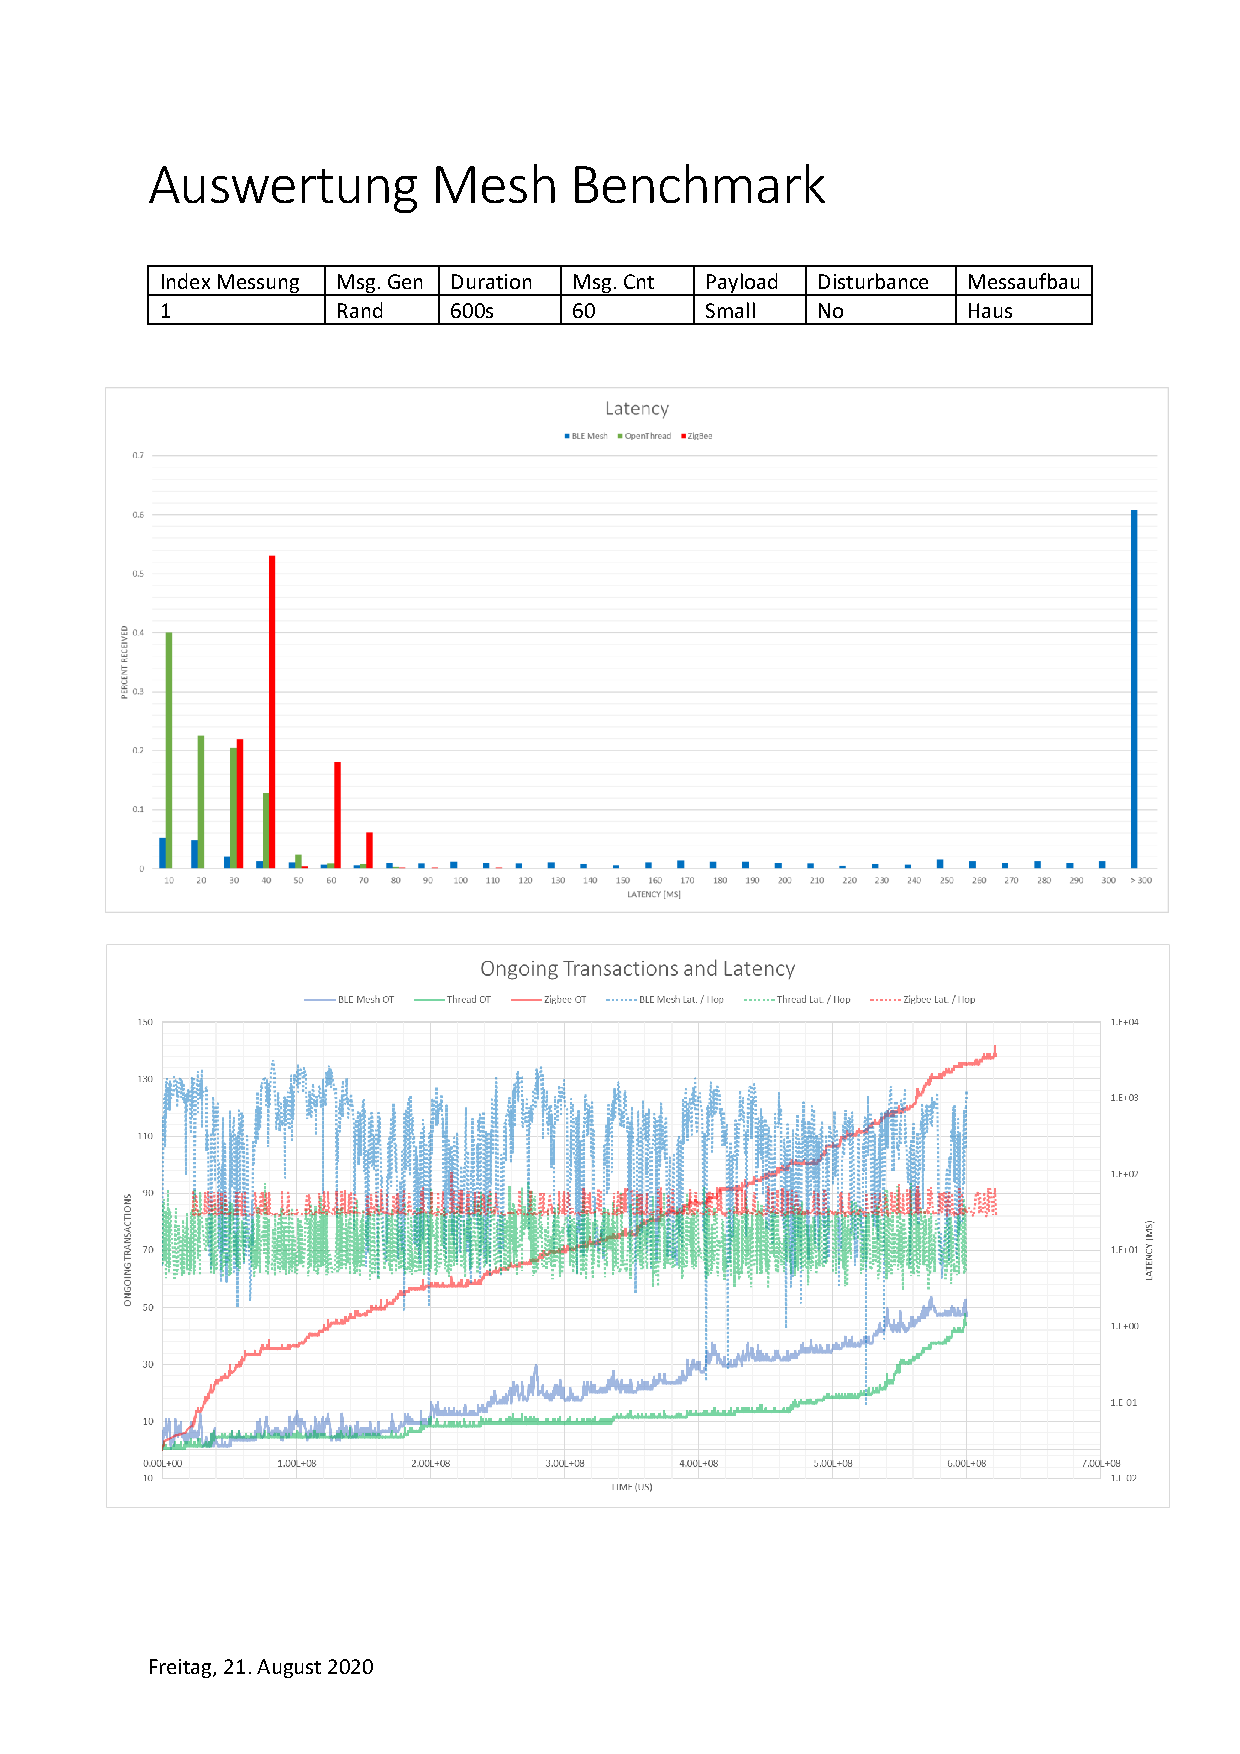
\includepdf[pages={1}, nup=1x1, landscape=false, scale=0.95 ,offset=0 0, pagecommand={\thispagestyle{myheadings}}]{appendix/Messprotokolle_Haus.pdf}

\includepdf[pages={2-8}, nup=1x1, landscape=false, scale=0.95 ,offset=0 0, pagecommand={\thispagestyle{myheadings}}]{appendix/Messprotokolle_Haus.pdf}

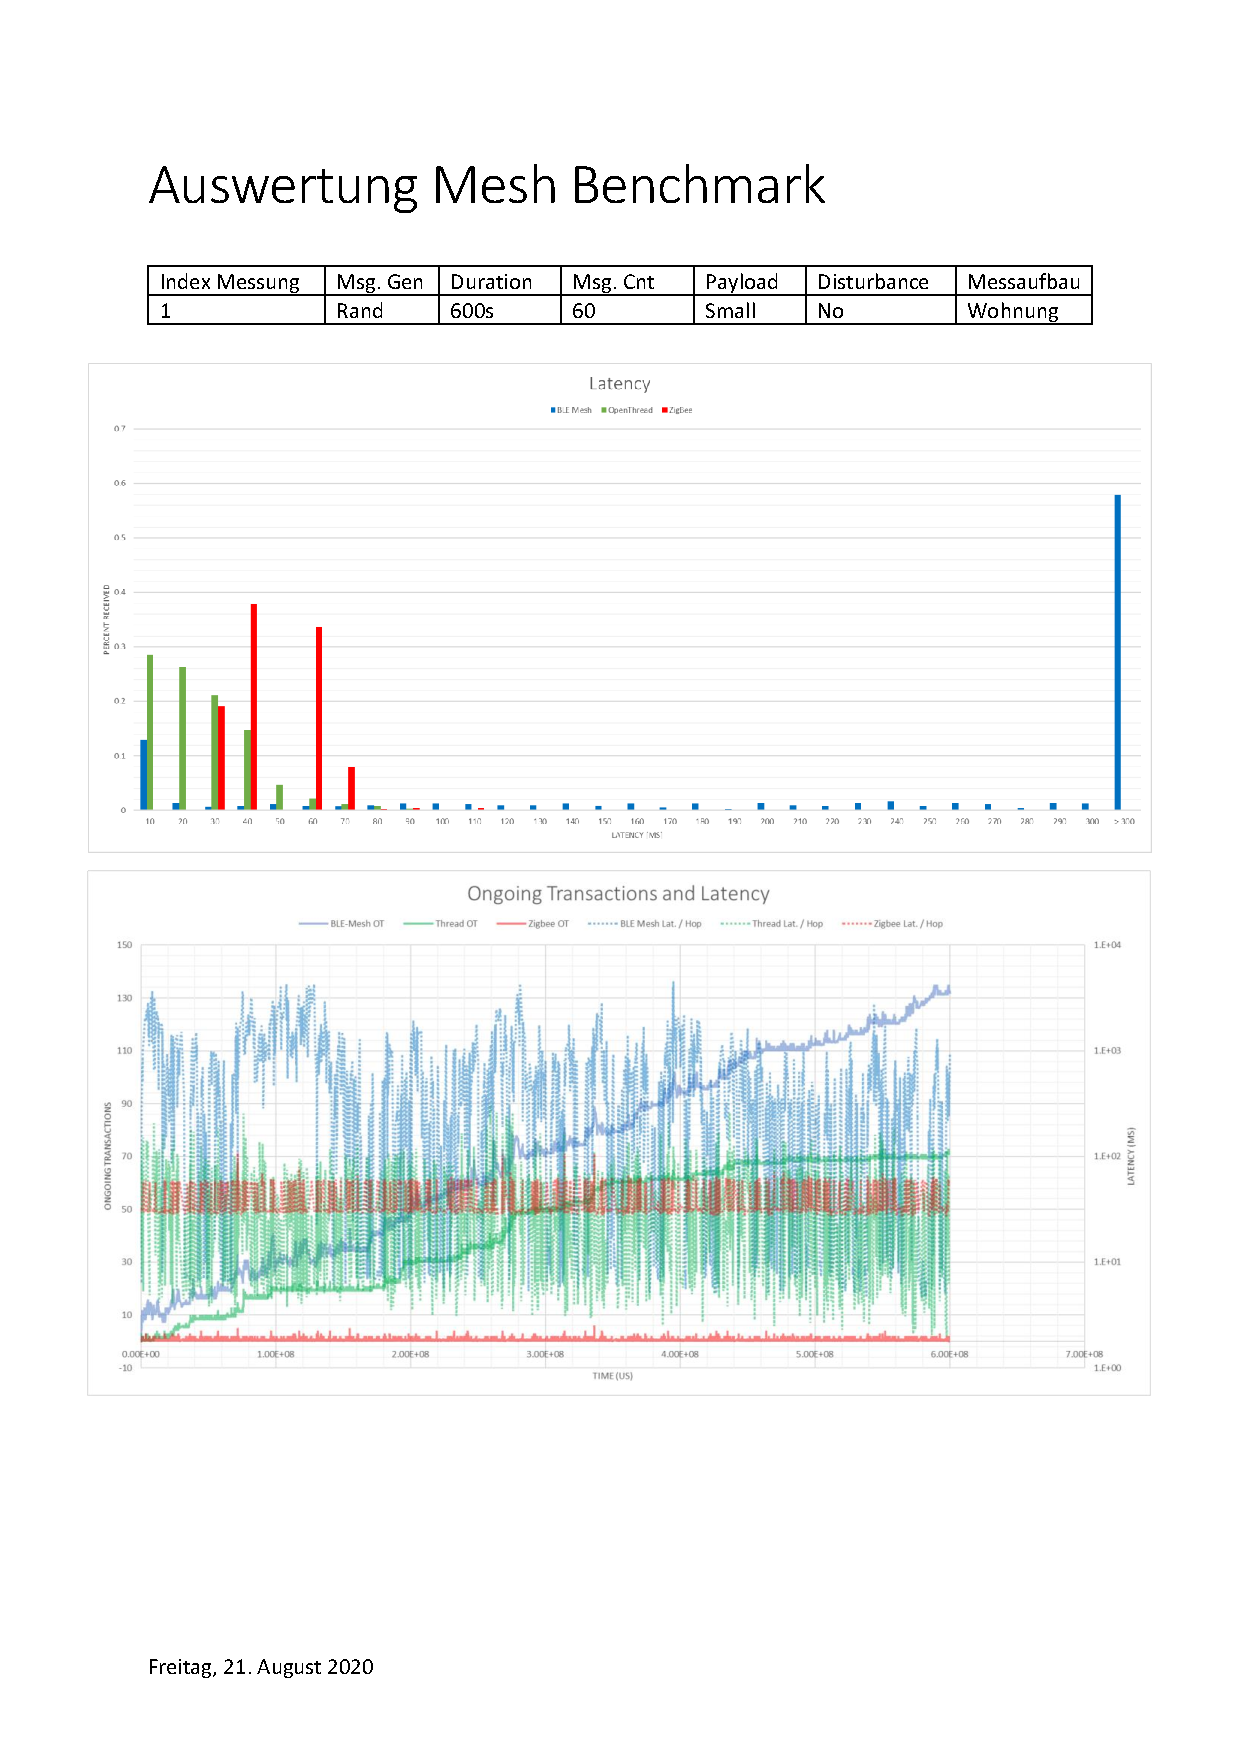
\includepdf[pages={1}, nup=1x1, landscape=false, scale=0.95 ,offset=0 0, pagecommand={\thispagestyle{myheadings}}]{appendix/Messprotokolle_Wohnung.pdf}

\includepdf[pages={2-8}, nup=1x1, landscape=false, scale=0.95 ,offset=0 0, pagecommand={\thispagestyle{myheadings}}]{appendix/Messprotokolle_Wohnung.pdf}

%***************Random Value Generation*********************
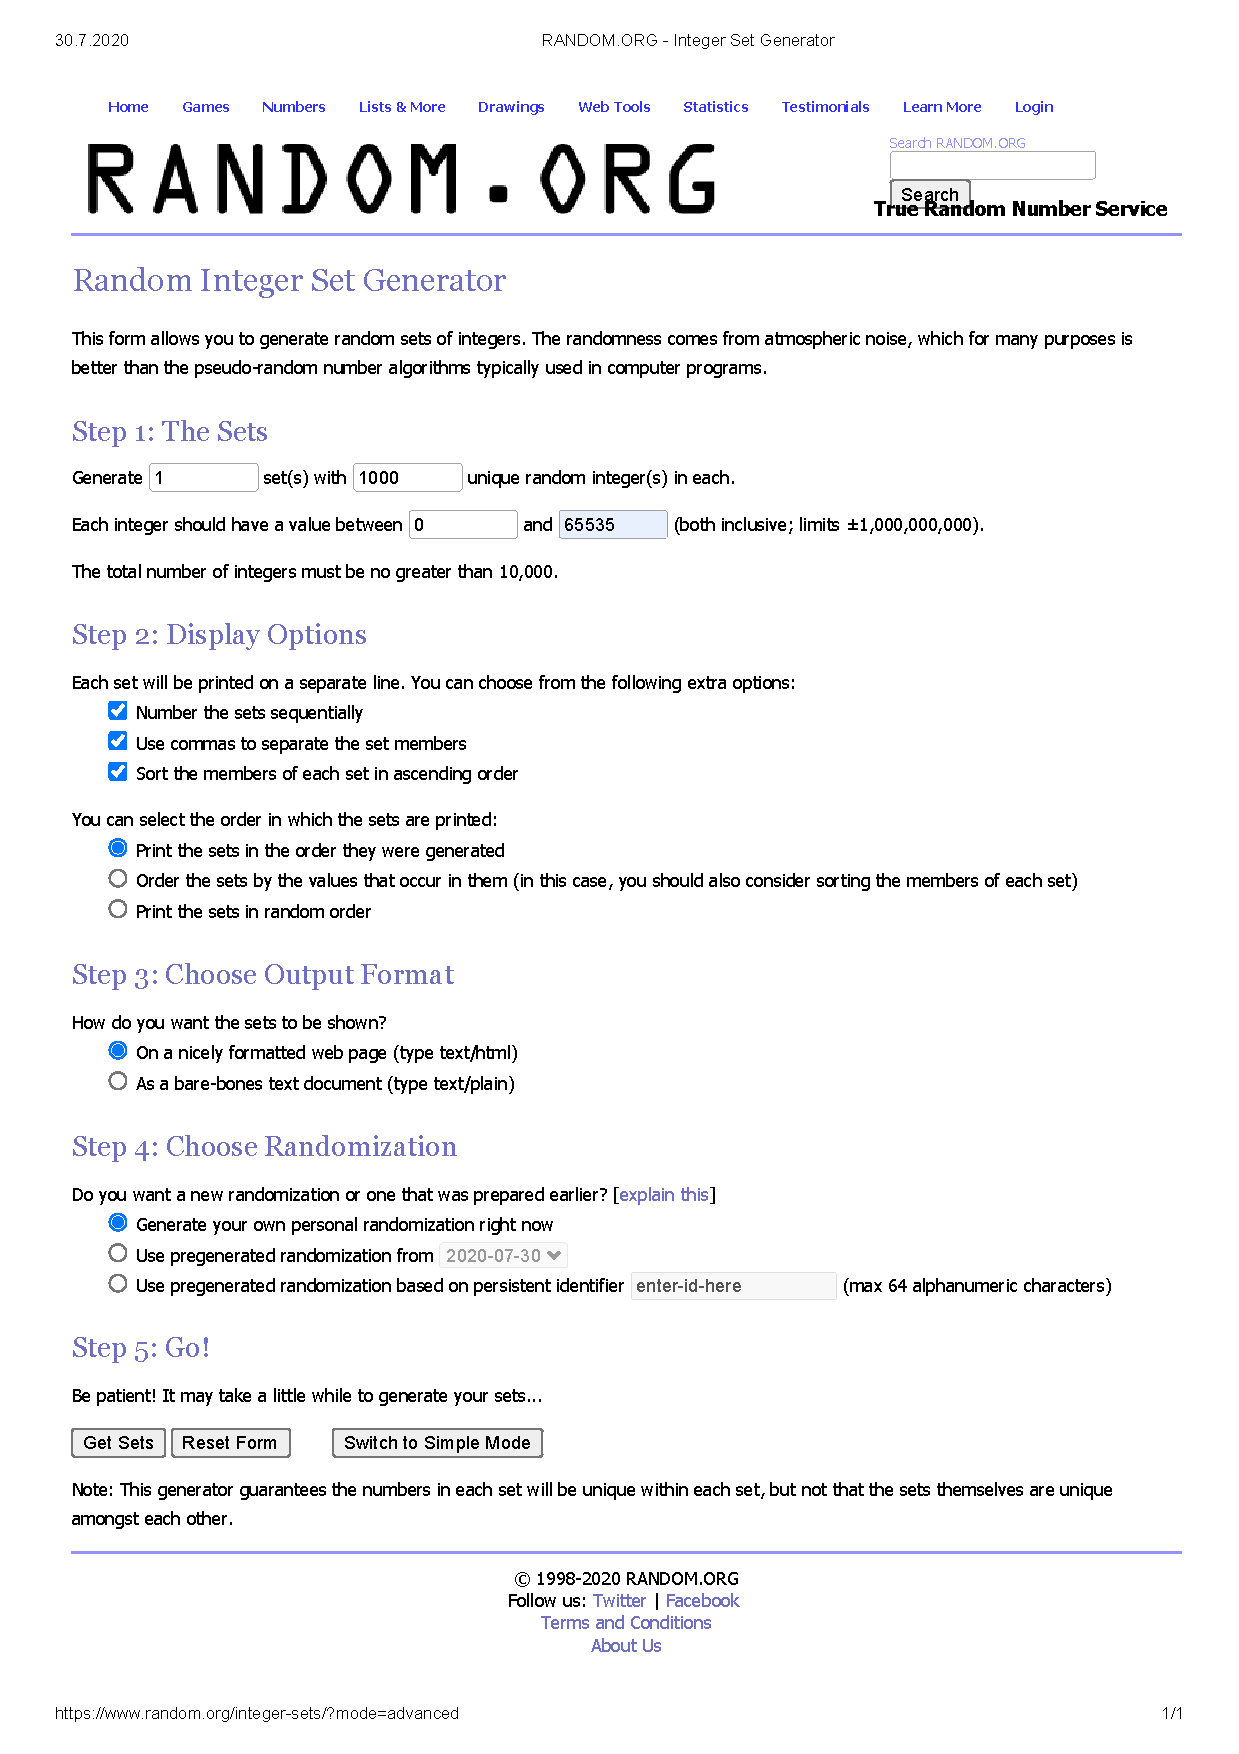
\includepdf[pages={1}, nup=1x1, landscape=false, scale=0.8 ,offset=0 -20, pagecommand={\section{Random Traffic Generation}\label{app:RandomTrafficGeneration}\thispagestyle{myheadings}}]{appendix/RANDOM.ORG_Integer_Set_Generator.pdf}


\end{appendix}



%%---NOTES for DEBUG---------------------------------------------------------------------
\ifdraft{%Do this only if mode=draft
%%requires \usepackage{todonotes})
\newpage
\listoftodos[\section{Todo-Notes}]
\clearpage
}
{%Do this only if mode=final
}

\end{document}
